\section{Flat plate}
The turbulent flow over a flat plate is investigated. All grids and results are available in~\cite{tmr} under the name: ``2D Zero pressure gradient flat plate''. The problem domain and flow conditions are shown in~\Cref{fig:flat}. NX Flow does not offer far-field BCs and uses an inlet BC on the leftmost face and openings on the top and rightmost face. Moreover, the problem was run with a fixed density in NX Flow so as to reduce computational cost, since this is essentially an incompressible case.

The Turbulence Modeling Resource provides five grids, each finer than the next, in order to compare so-called mesh independent results and to perform a grid study. The goal of a grid study is to establish that the obtained results will not vary significantly by further refining the mesh, and thus that the obtained results are as accurate as possible.
\begin{figure}
    \centering
    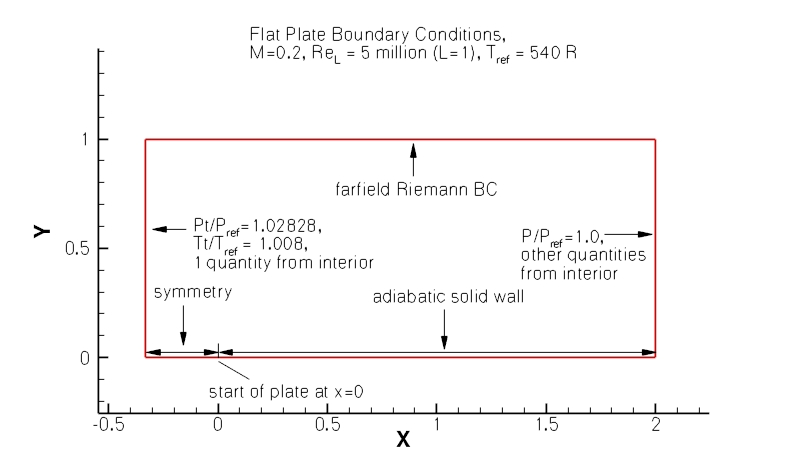
\includegraphics[width=0.7\textwidth]{figs/flat/flatplate.png}
    \caption{Turbulent flat plate case~\cite{tmr}.}
    \label{fig:flat}
\end{figure}

The skin friction coefficient $C_f$ at $x = 0.97$ and drag coefficient $C_D$ are compared to CFL3D, a cell-centered finite volume code developed by NASA, in~\Cref{tab:flat}. These coefficients are calculated as:
\begin{align*}
    C_f = \frac{2\tau_w}{\rho_\infty U_\infty^2}\\
    C_D = \frac{2D}{\rho_\infty U_\infty^2 A},
\end{align*}
where $D$ is the drag force and $A$ the reference area. For this case, the reference area is the length of the plate times its width, i.e. the length of the mesh in the $z$ direction. \Cref{tab:flat} tabulates the skin friction coefficient and drag coefficient values.
All values are within 2\% of each other. Reasons for discrepancies are given below.
\begin{table}
\centering
\caption{Flat Plate (syn3D \& NX Flow): Comparison of force coefficients on the finest grid.}
\label{tab:flat}
\begin{tabular}{@{}lcc@{}}
    \toprule
    Solver & $C_D$ & $C_f$ at $x=0.97$ \\
    \midrule
    CFL3D & 0.00286 & 0.00270 \\
    NX Flow & 0.00288 & 0.00272 \\
    syn3D & 0.00280 & 0.00269\\
    \bottomrule
\end{tabular}
\end{table}
\Cref{fig:synflatcnvstudy} shows the residual convergence of the density residual and turbulence residual for all grids with syn3D. \Cref{fig:nxflatcnvstudy} shows the residual of all equations for all grids with NX Flow. As expected, the coarser grids show faster convergence than the finer ones -- this phenomenon is detailed in~\cite{blazek2015computational}. While the residual was never driven down to machine precision, differences in the obtained solution field were found to be marginal by further reducing the residual.

\Cref{tab:flatcpu} compares the number of iterations and CPU time between syn3D and NX Flow for the medium grid, which demonstrates the advantages of an implicit solver over an explicit solver: around two thousand times more iterations are taken by syn3D. On the other hand, explicit iterations are much less computationally expensive and require less storage. It should also be noted that NX Flow does not solve the conservation of energy equation for this particular case, since it uses a fixed density. Moreover, multigrid was not used with syn3D for this case, which significantly accelerates convergence in most cases.
\begin{table}
\caption{Flat Plate (syn3D \& NX Flow): Convergence metrics on the medium grid.}
\label{tab:flatcpu}
\begin{tabular}{@{}l ccccc@{}}
\toprule
Solver & Processors & Iterations & Time taken & Time per iteration & Residual reduction \\
       &            &            & (min)      & (sec)              &                    \\
\midrule
% NX Flow (4 cores) & 205 & 34 & $\approx$ 10 & $10^{-10}$ \\
% syn3D (8 cores) & 400000 & 156 & $\approx$ 0.023 & $10^{-8}$
NX Flow & 4 & 205 & 34 & $\approx$ 10 & $10^{-10}$ \\
syn3D & 8 & 400000 & 156 & $\approx$ 0.023 & $10^{-8}$
\\
\bottomrule
\end{tabular}
\end{table}

\begin{figure}[ht!]
\centering
\begin{subfigure}{.45\textwidth}
  \centering
  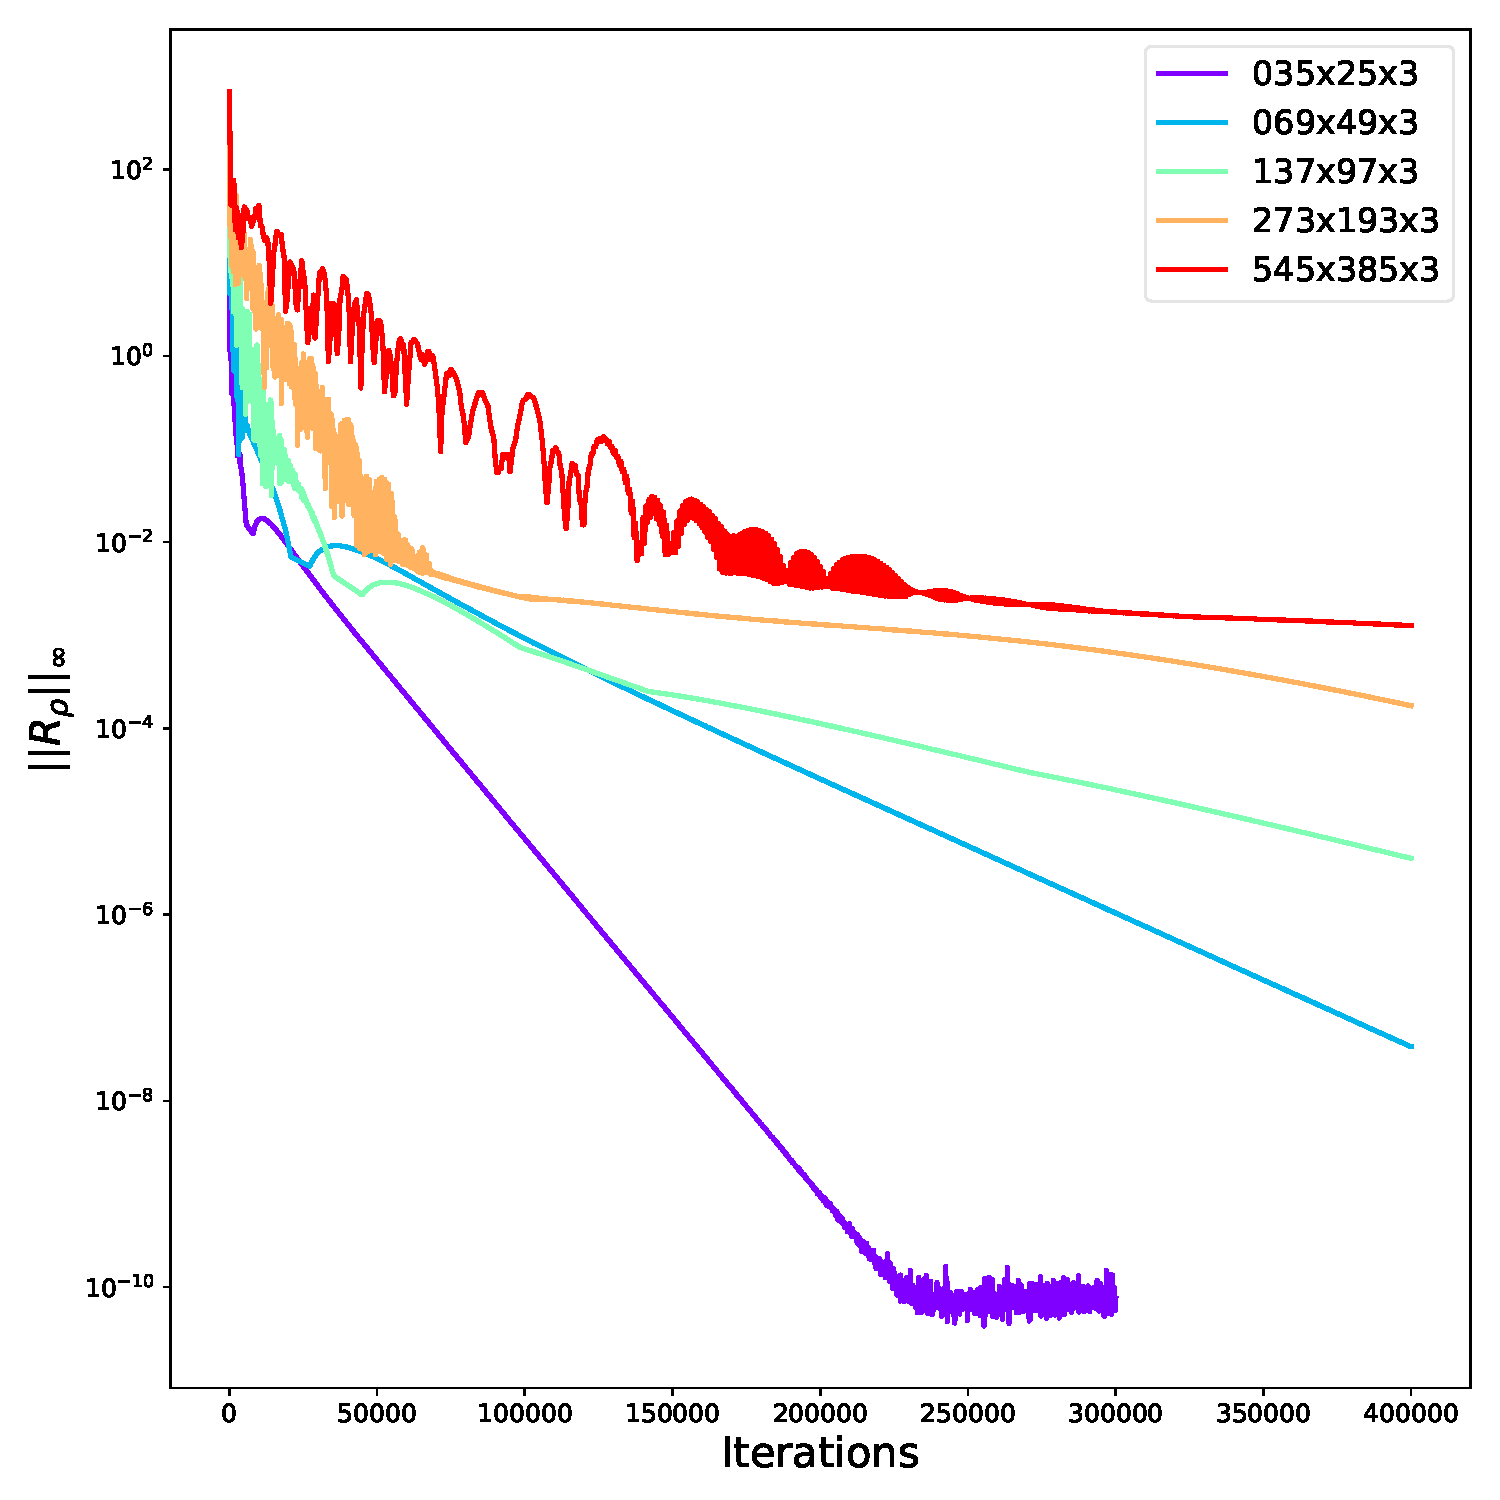
\includegraphics[width=1.0\textwidth]{figs/flat/gov_convergence_gridstudy.pdf}
  \caption{Maximum density residual.}
\end{subfigure}%
\begin{subfigure}{.45\textwidth}
    \centering
    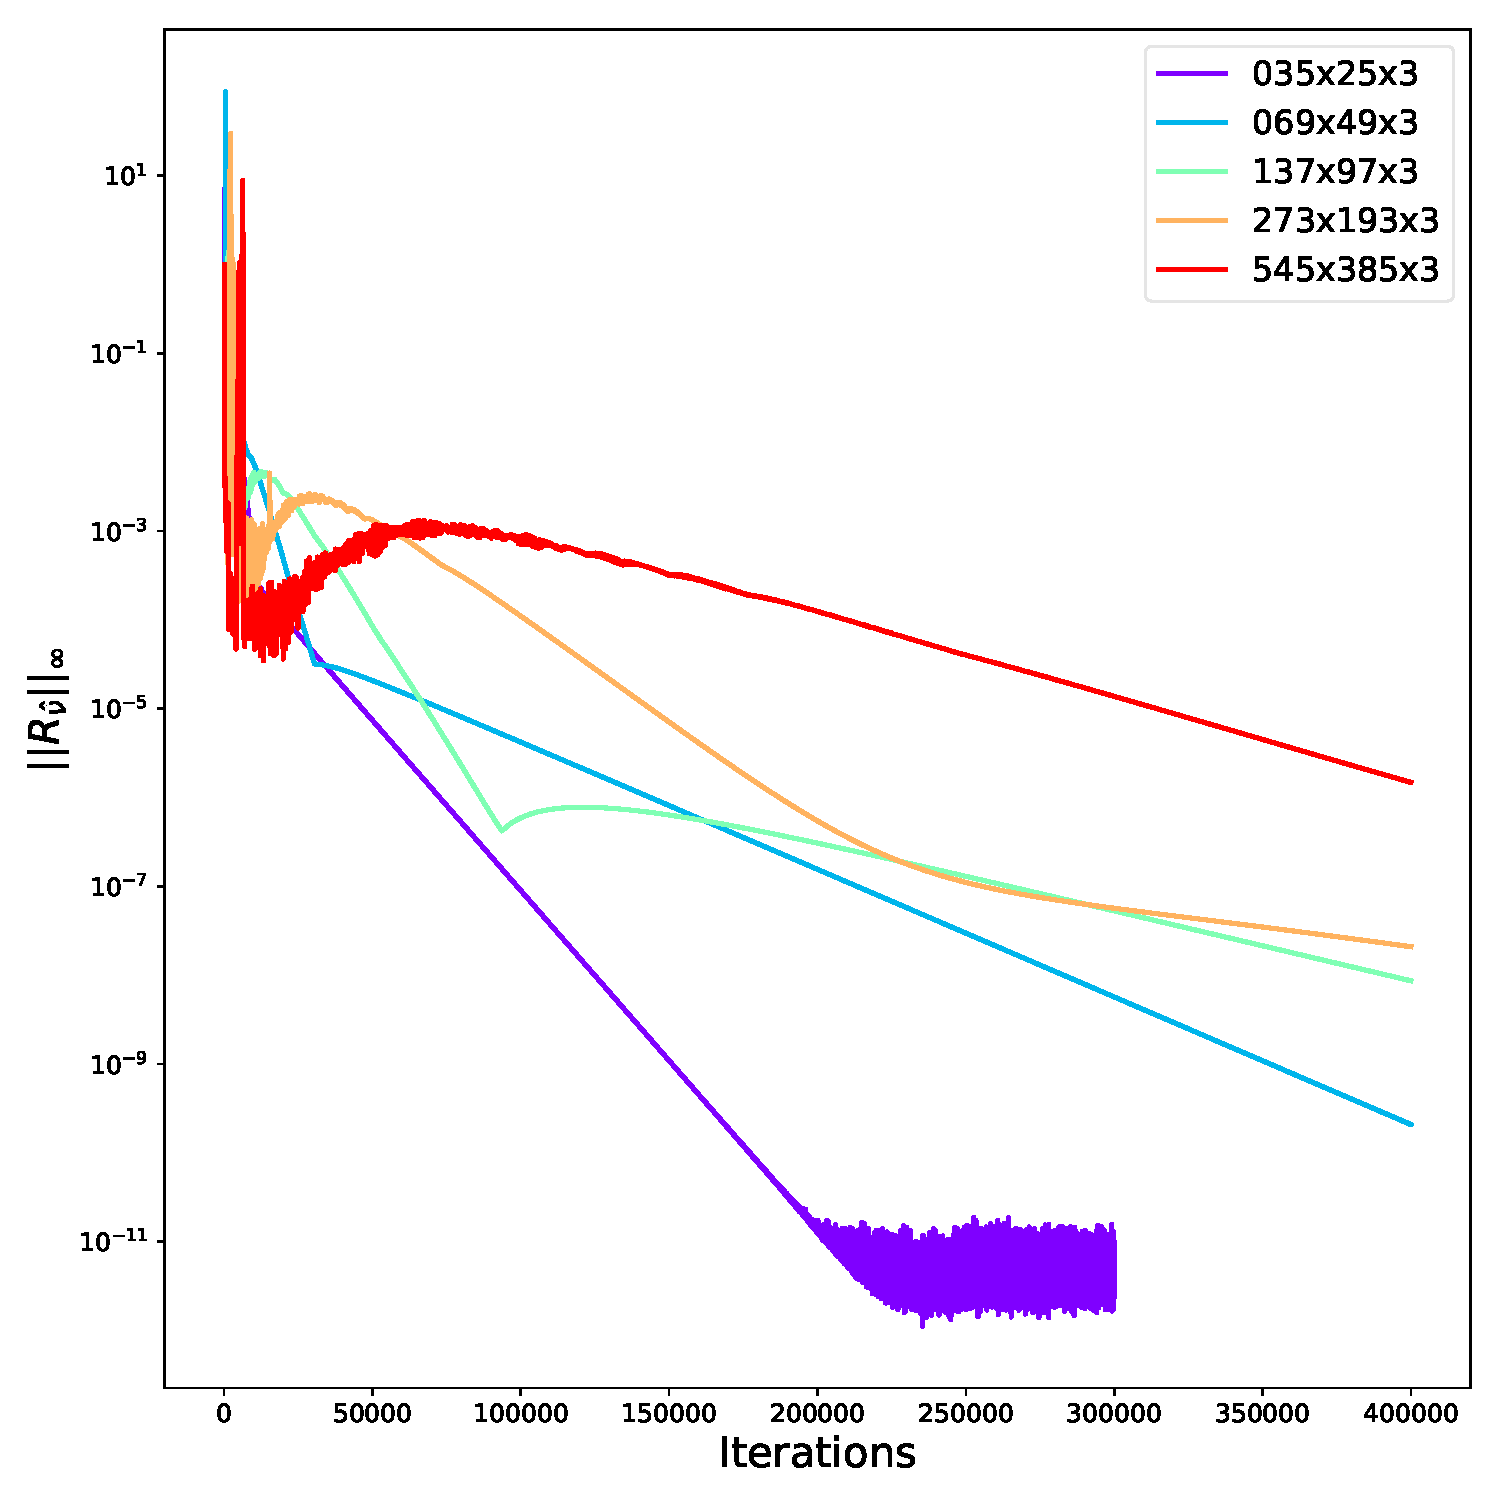
\includegraphics[width=1.0\textwidth]{figs/flat/SA_convergence_gridstudy.pdf}
    \caption{Maximum turbulence variable residual.}
\end{subfigure}
\caption{Flat Plate (syn3D): Convergence of flow and turbulence variables on various grid sizes.}
\label{fig:synflatcnvstudy}
\end{figure}
\begin{figure}[ht!]
    \centering
    \begin{subfigure}{0.48\textwidth}
        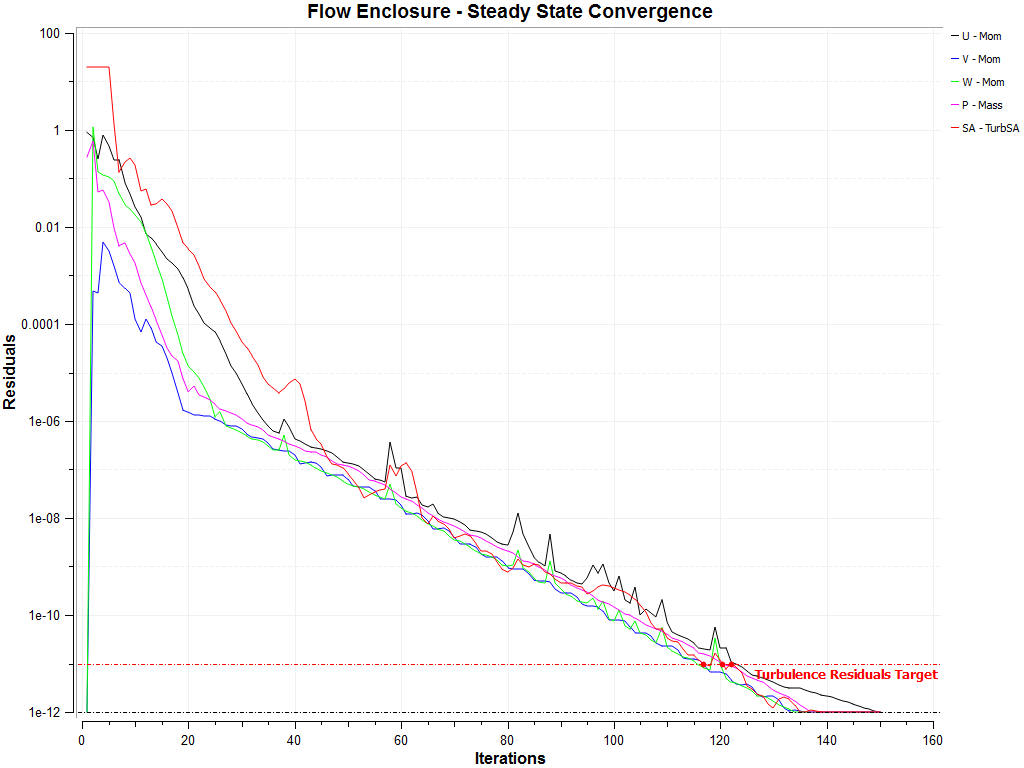
\includegraphics[width=\textwidth]{./figs/flatnx/35x25_conv.png}
        \caption{35x25}
    \end{subfigure}
    \hfill
    \begin{subfigure}{0.48\textwidth}
        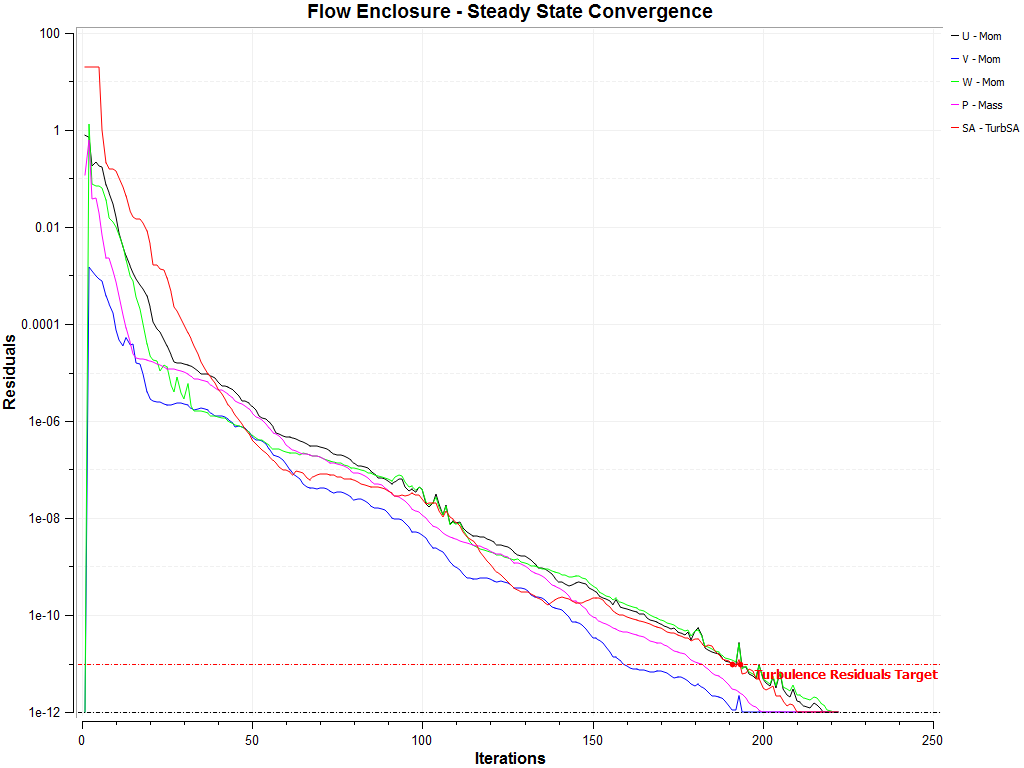
\includegraphics[width=\textwidth]{./figs/flatnx/69x49_conv.png}
        \caption{69x49}
    \end{subfigure}
    \\
    \begin{subfigure}{0.48\textwidth}
        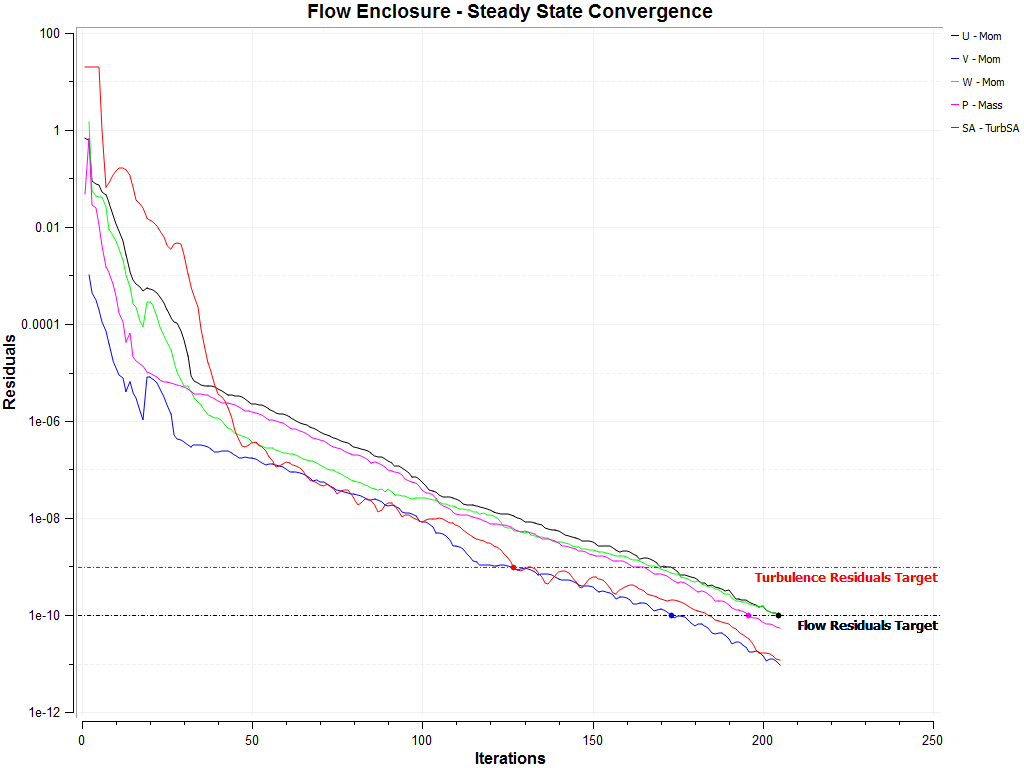
\includegraphics[width=\textwidth]{./figs/flatnx/137x97_conv.png}
        \caption{137x97}
    \end{subfigure}
    \hfill
    \begin{subfigure}{0.48\textwidth}
        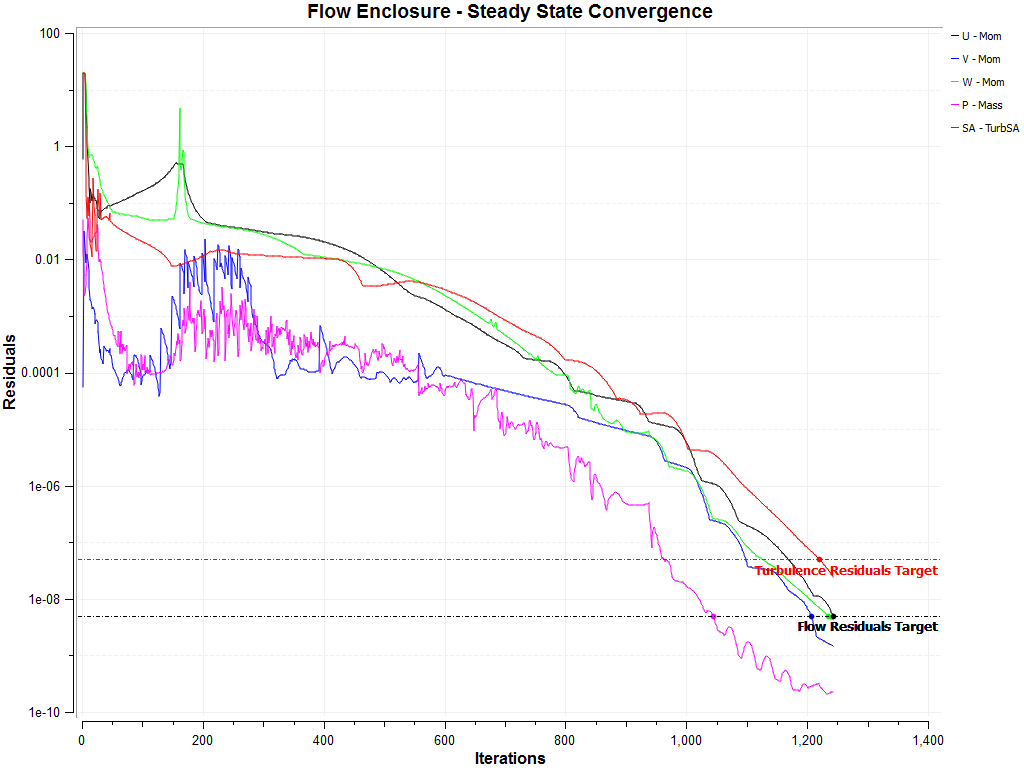
\includegraphics[width=\textwidth]{./figs/flatnx/273x193_conv.png}
        \caption{273x193}
    \end{subfigure}
    \\
    \begin{subfigure}{0.48\textwidth}
        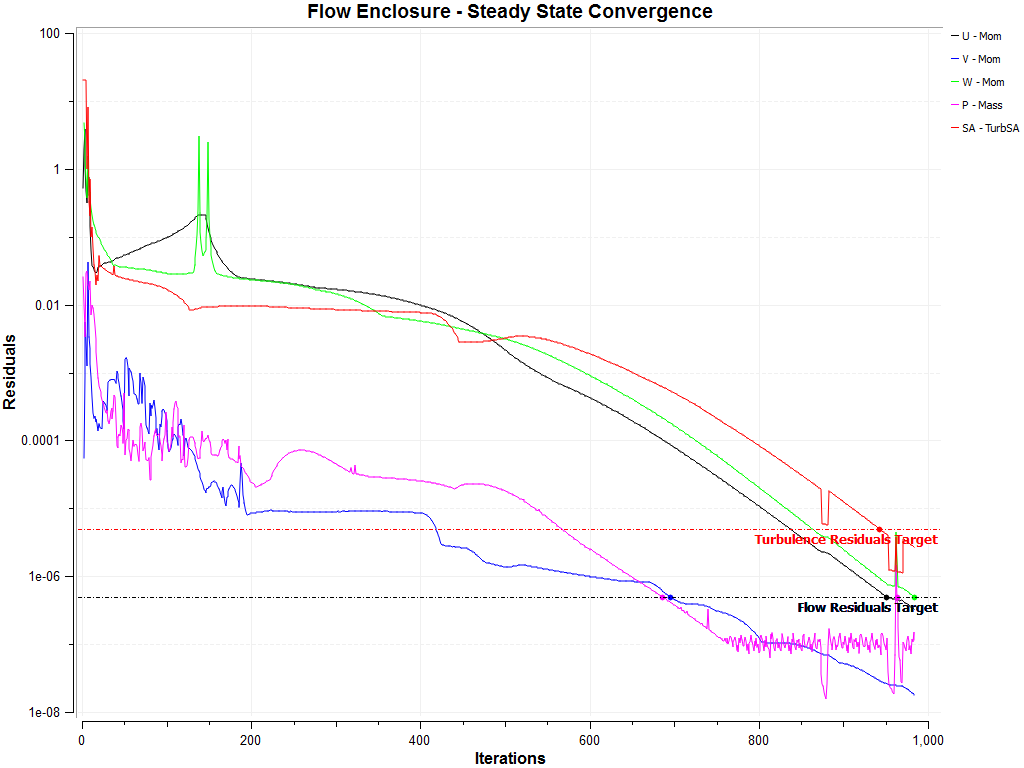
\includegraphics[width=\textwidth]{./figs/flatnx/545x385_conv.png}
        \caption{545x385}
    \end{subfigure}
    \caption{Flat Plate (NX Flow): Convergence of residuals on various grid sizes.}
    \label{fig:nxflatcnvstudy}
\end{figure}

Several plots have been generated to compare the results between all solvers. Unless otherwise noted, all results were obtained with the finest grid. \Cref{fig:flatcf} compares the skin friction along the plate, which is maximal at the leading edge and then gradually decreases. NX Flow and syn3D display slight over-prediction and under-prediction respectively. The skin friction coefficient is a measure of the velocity gradient at the wall.

\Cref{fig:flatmutcontour} shows contour plots of the dimensionless eddy viscosity $\frac{\mu_t}{\mu_{\infty}}$ and \Cref{fig:flatmu} shows line plots of the dimensionless eddy viscosity. As expected, the eddy viscosity increases gradually as the wall distance increases, as turbulence effects are more significant in the log-law region, and then diminishes as it reaches the far-field region. This is in accordance with the law of the wall, which states that turbulent stresses are minimal in the viscous sublayer and maximal in the log-law layer. Moreover, the eddy viscosity, initially close to zero, increases with $x$ due to production near the wall as well as advection.

\Cref{fig:flatu,fig:flatupyp} show profiles of the dimensionless velocity $u/u_\infty$ and $u^+$ respectively. The velocity profile shows a sharp gradient near the wall, typical of turbulent flows. Moreover, the height of the boundary layer, the region where velocity is reduced as compared to the far-field, grows with increasing $x$. It can also be seen that the $u^+$ profile agrees with the theory: $u^+$ follows the $u^+=y^+$ curve in the viscous sublayer and the log-law curve in the log-law region.

Overall, there is excellent agreement between NX Flow and CFL3D and some level of discrepancy between syn3D and CFL3D. The source of discrepancy is easily seen in~\Cref{fig:flatmutmax}: the eddy viscosity jumps abruptly right at the leading edge for syn3D but not for the other two. It should be noted that the spike occurs at the interface between block boundaries, which could be the cause of this phenomenon. These blocks thus have different boundary conditions at their $y=0$ face. Moreover, the jump does not occur if the domain only includes the plate, i.e. starts at $x=0$.
% The cause of this jump was investigated by the author as well as others working on the code, but a definite answer was unfortunately not found.
\begin{figure}[ht!]
\centering
	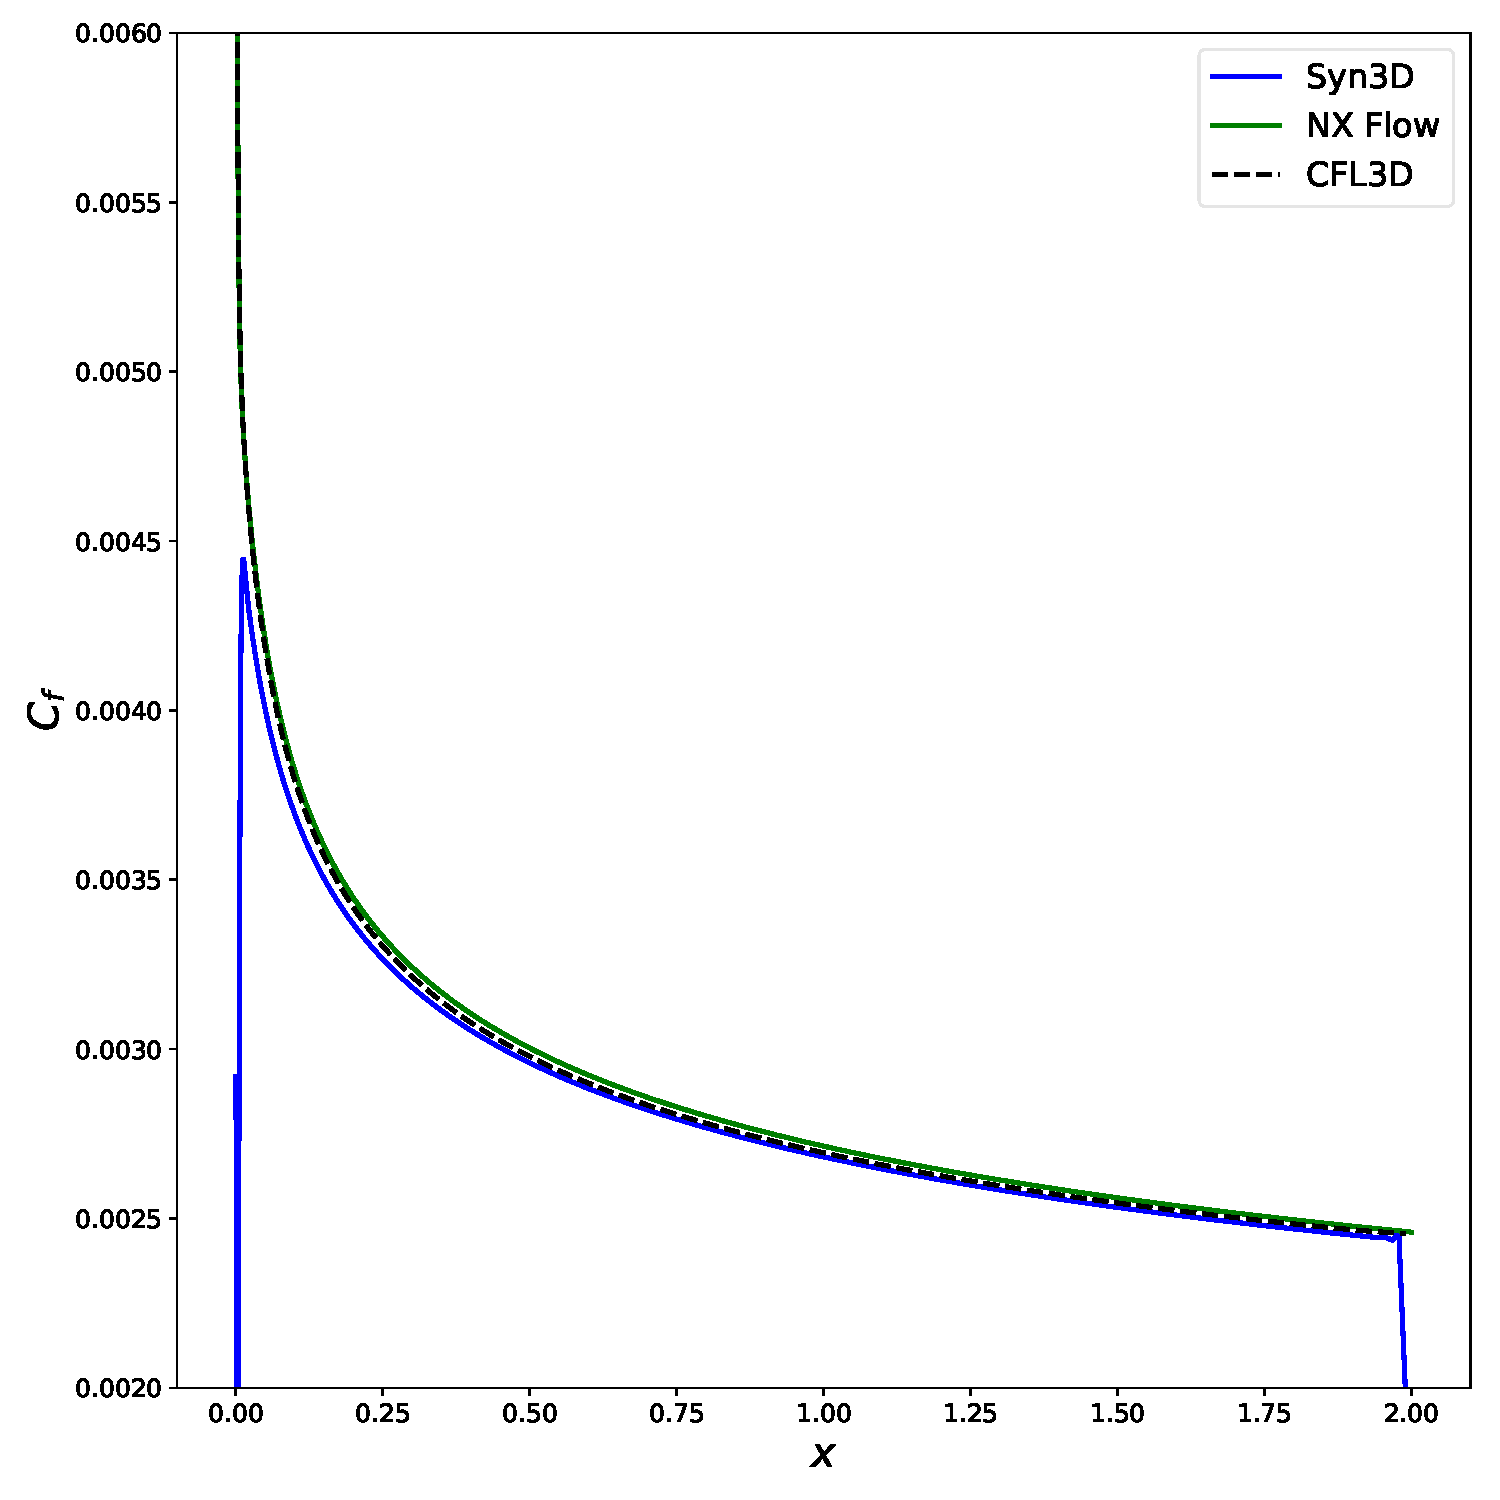
\includegraphics[width=0.7\textwidth]{figs/flat/skin_friction.pdf}
    \caption{Flat Plate (syn3D \& NX Flow): Coefficient of skin friction along the plate.}
    \label{fig:flatcf}
\end{figure}

\begin{figure}[ht!]
\centering
\begin{subfigure}{.32\textwidth}
  \centering
  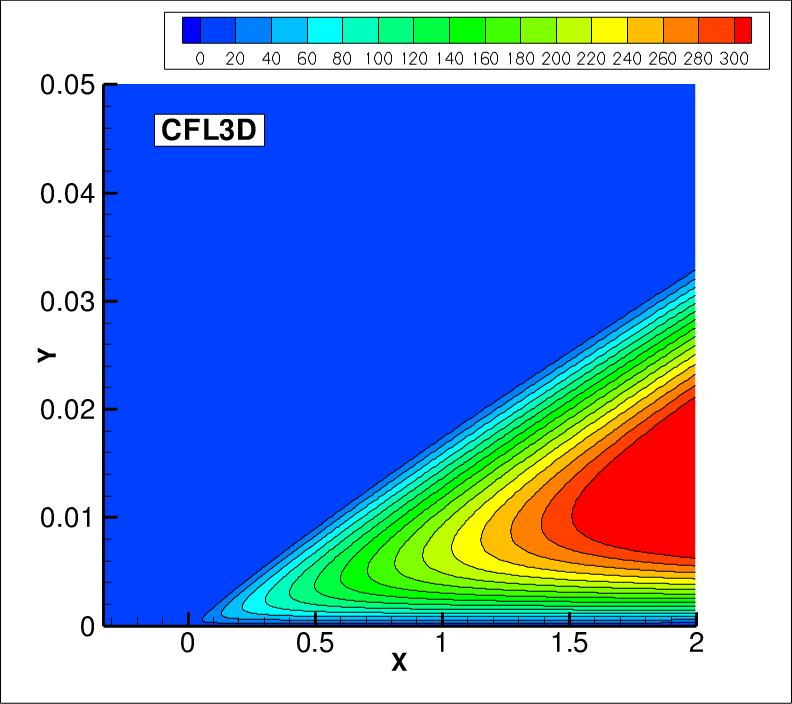
\includegraphics[width=1.0\textwidth]{figs/flat/mut_contours_cfl3d.jpg}
  \caption{CFL3D}
\end{subfigure}%
\begin{subfigure}{.32\textwidth}
  \centering
  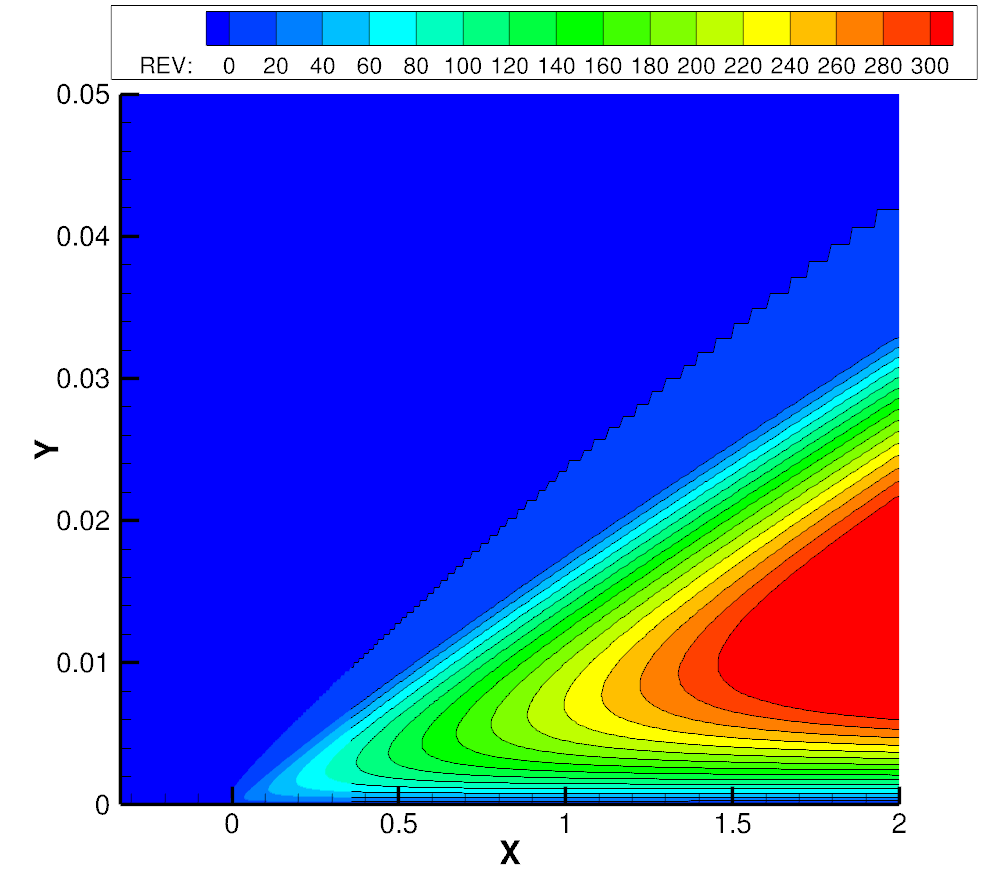
\includegraphics[width=1.0\textwidth]{figs/flat/rev_sa.png}
  \caption{syn3D}
\end{subfigure}
\begin{subfigure}{.32\textwidth}
  \centering
  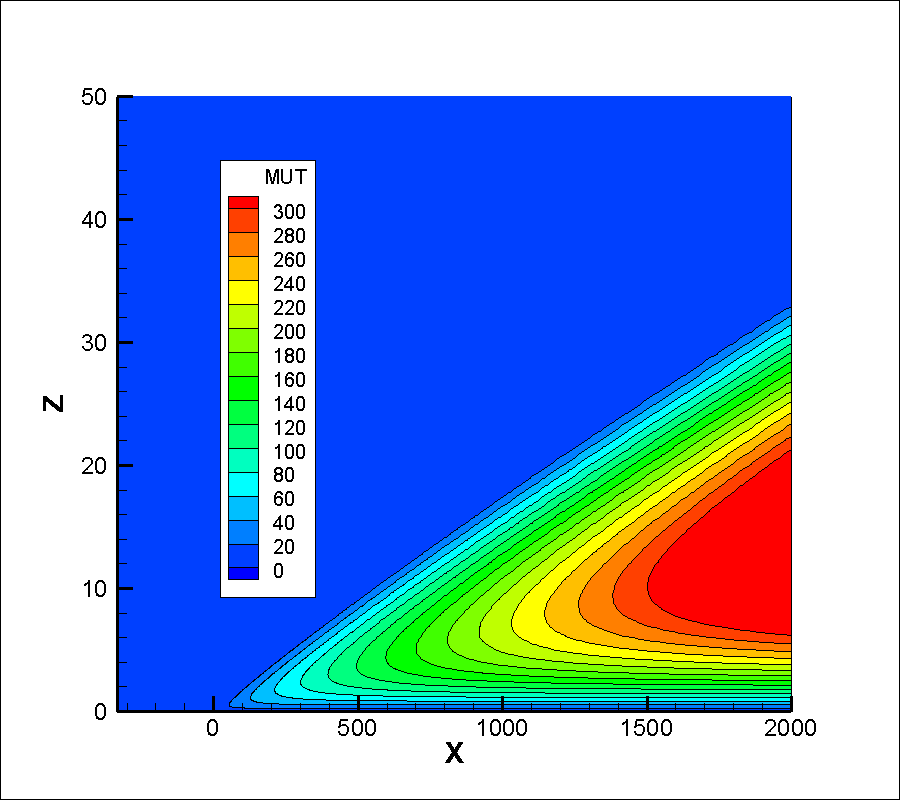
\includegraphics[width=1.0\textwidth]{figs/flatnx/mut_contour.png}
  \caption{NX Flow}
\end{subfigure}
\caption{Flat Plate (syn3D \& NX Flow): Contours of dimensionless eddy viscosity}
\label{fig:flatmutcontour}
\end{figure}

\begin{figure}[ht!]
\centering
\begin{subfigure}{.45\textwidth}
  \centering
  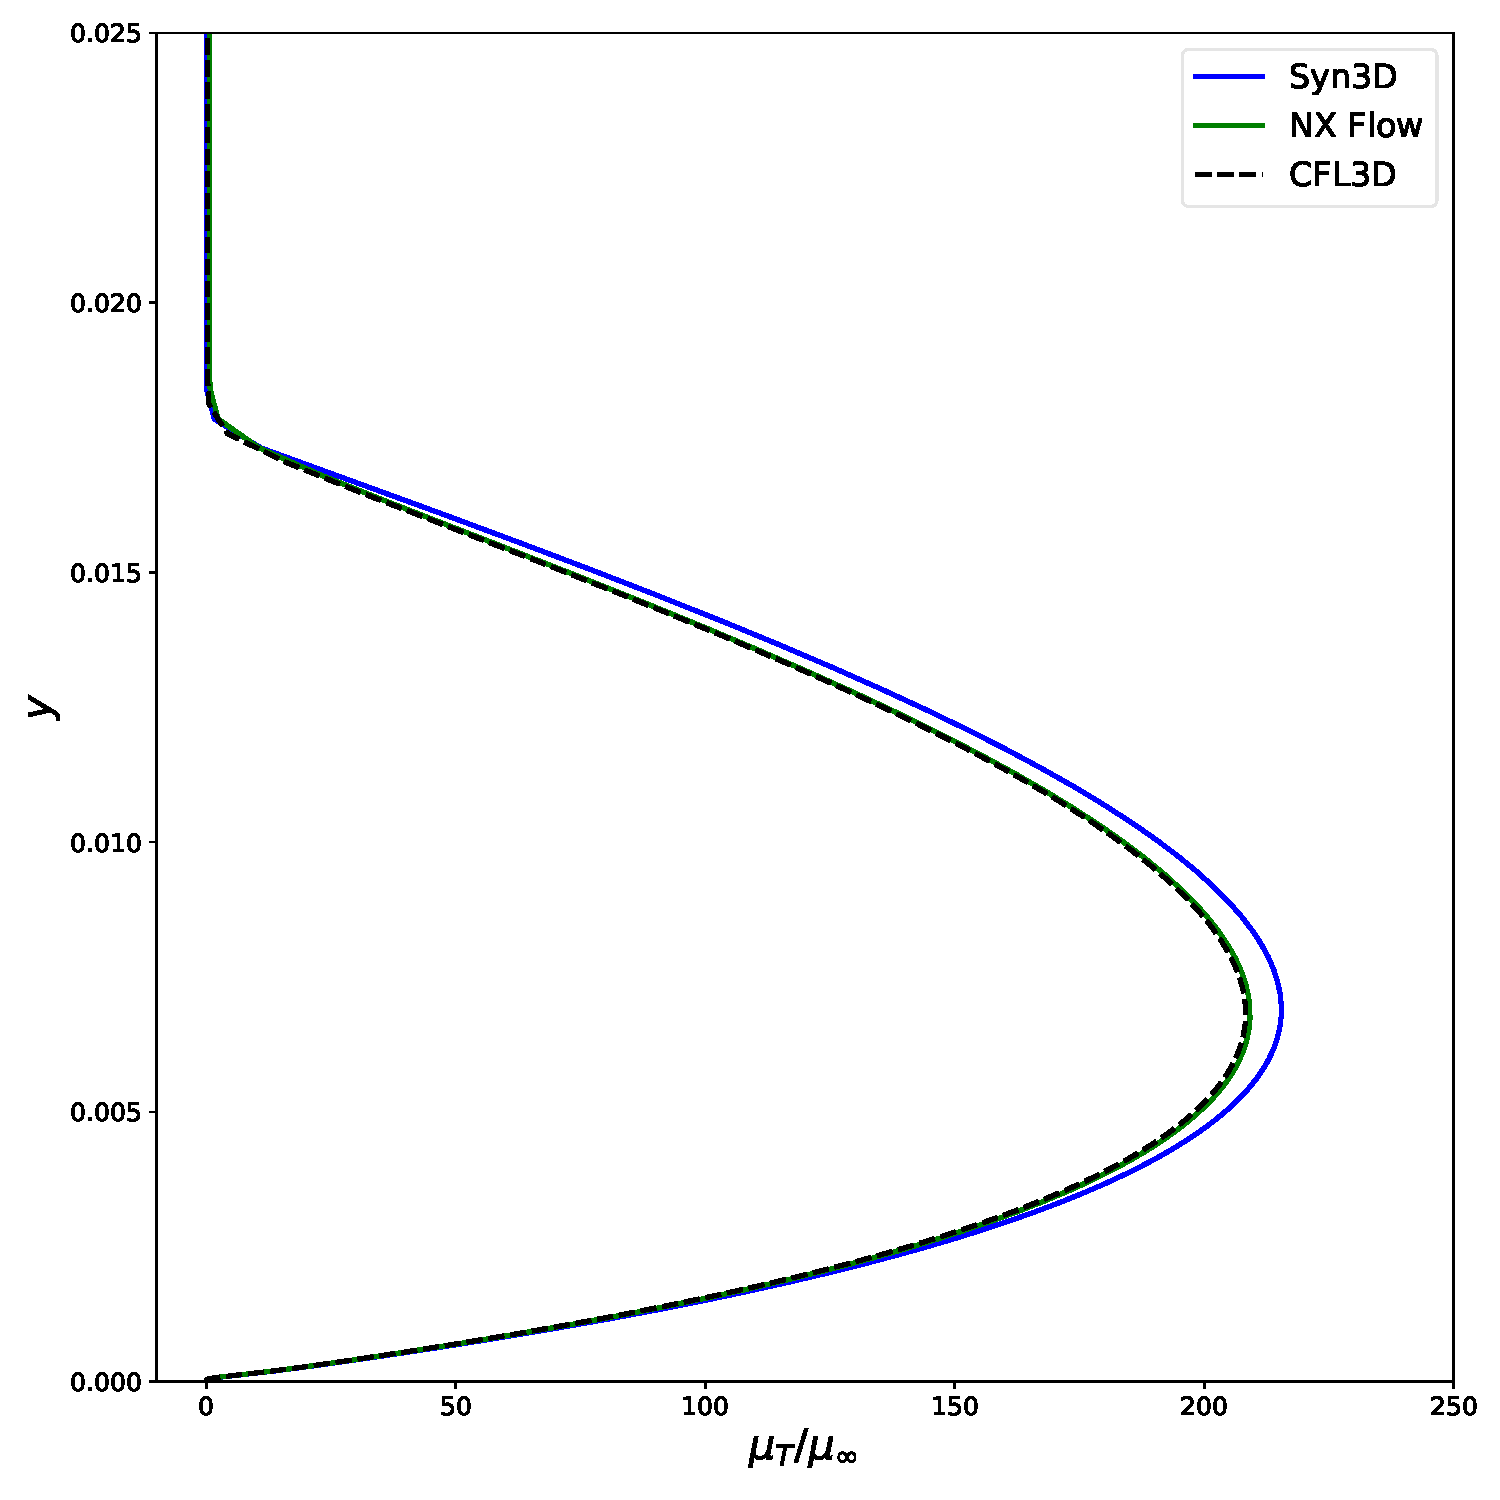
\includegraphics[width=1.0\textwidth]{figs/flat/mut_x097.pdf}
  \caption{Nondimensional eddy viscosity at x=0.97 }
\end{subfigure}%
\begin{subfigure}{.45\textwidth}
  \centering
  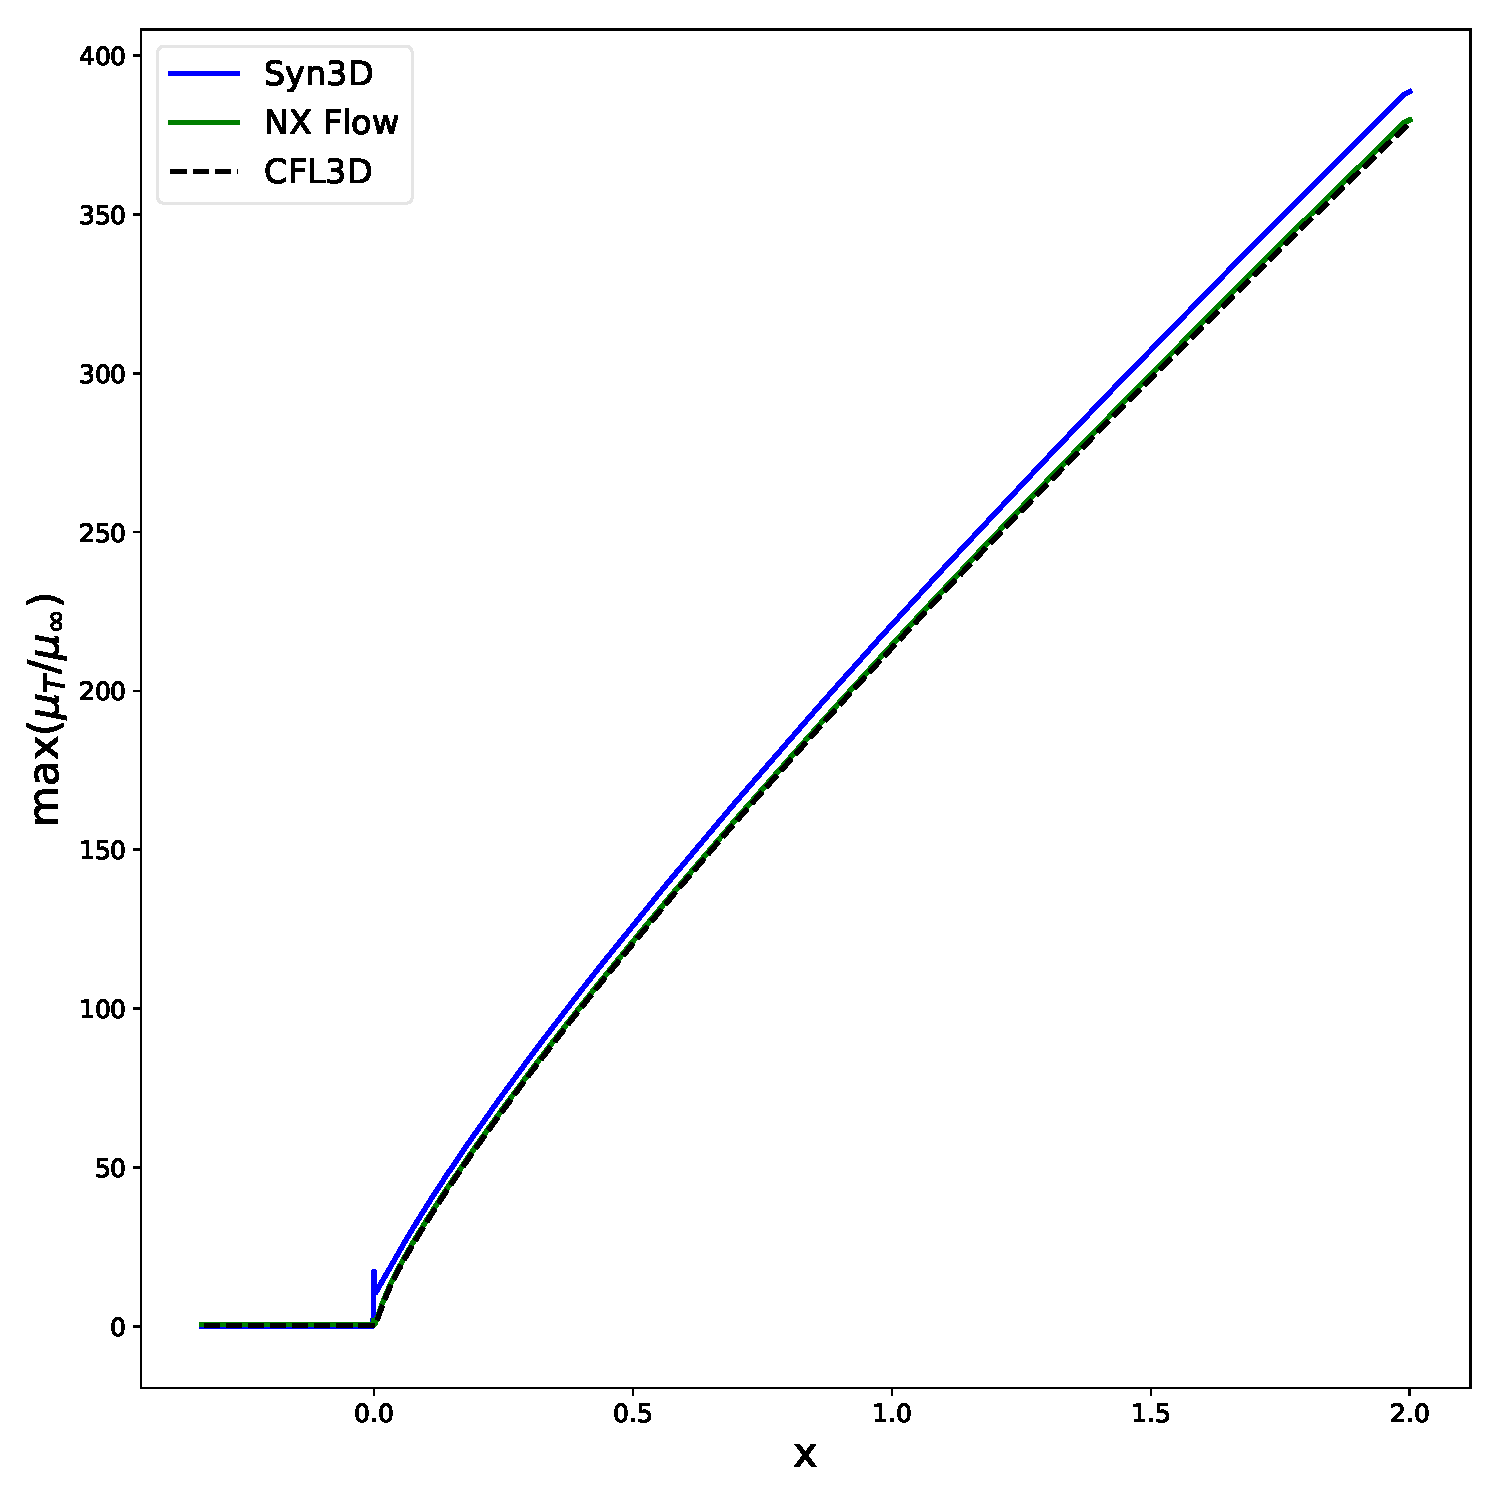
\includegraphics[width=1.0\textwidth]{figs/flat/maxmut.pdf}
  \caption{Maximum $\frac{\mu_t}{\mu_{\infty}}$ in the boundary layer}
  \label{fig:flatmutmax}
\end{subfigure}
\caption{Flat Plate (syn3D \& NX Flow): Dimensionless eddy viscosity line plots}
\label{fig:flatmu}
\end{figure}

\begin{figure}[ht!]
\centering
\begin{subfigure}{.45\textwidth}
  \centering
  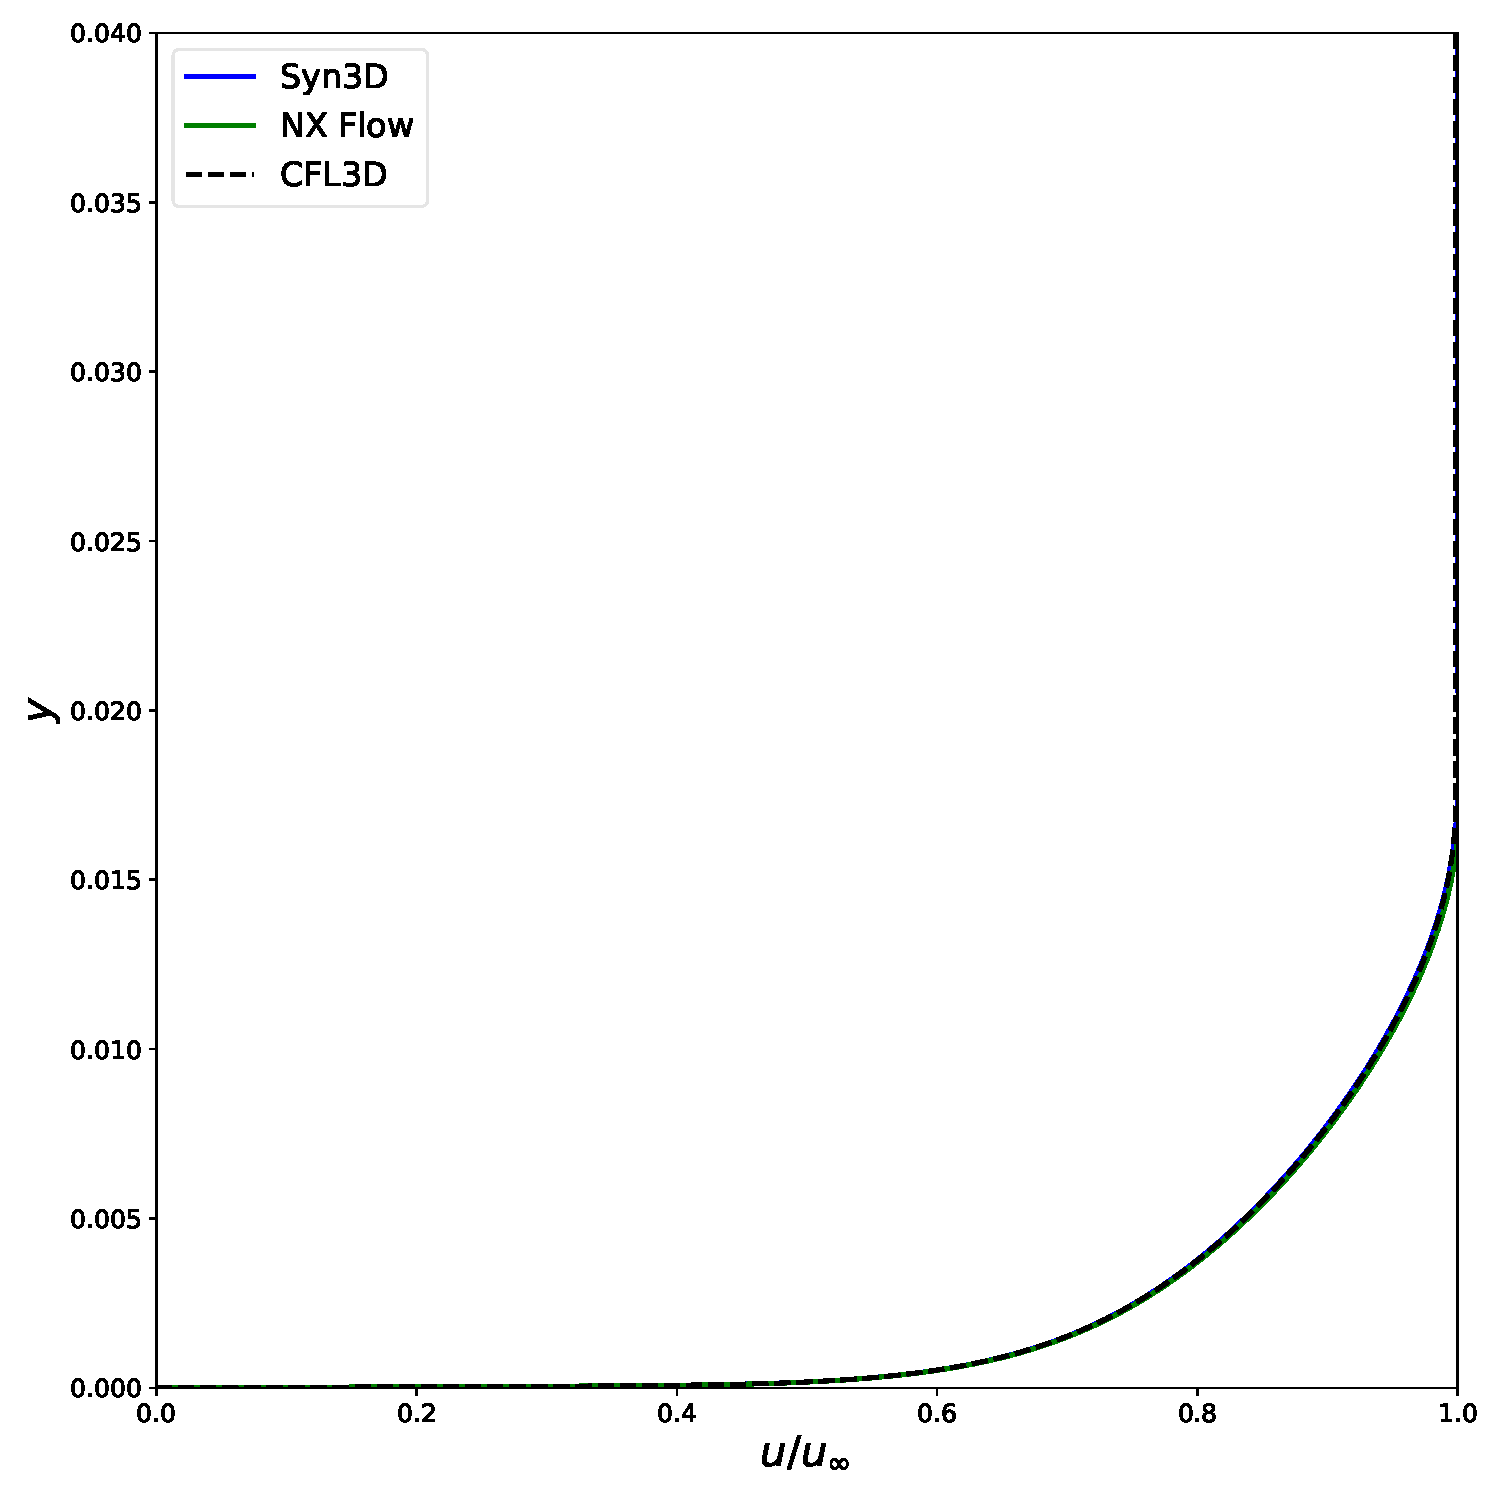
\includegraphics[width=1.0\textwidth]{figs/flat/u097.pdf}
  \caption{$x=0.97$}
\end{subfigure}%
\begin{subfigure}{.45\textwidth}
  \centering
  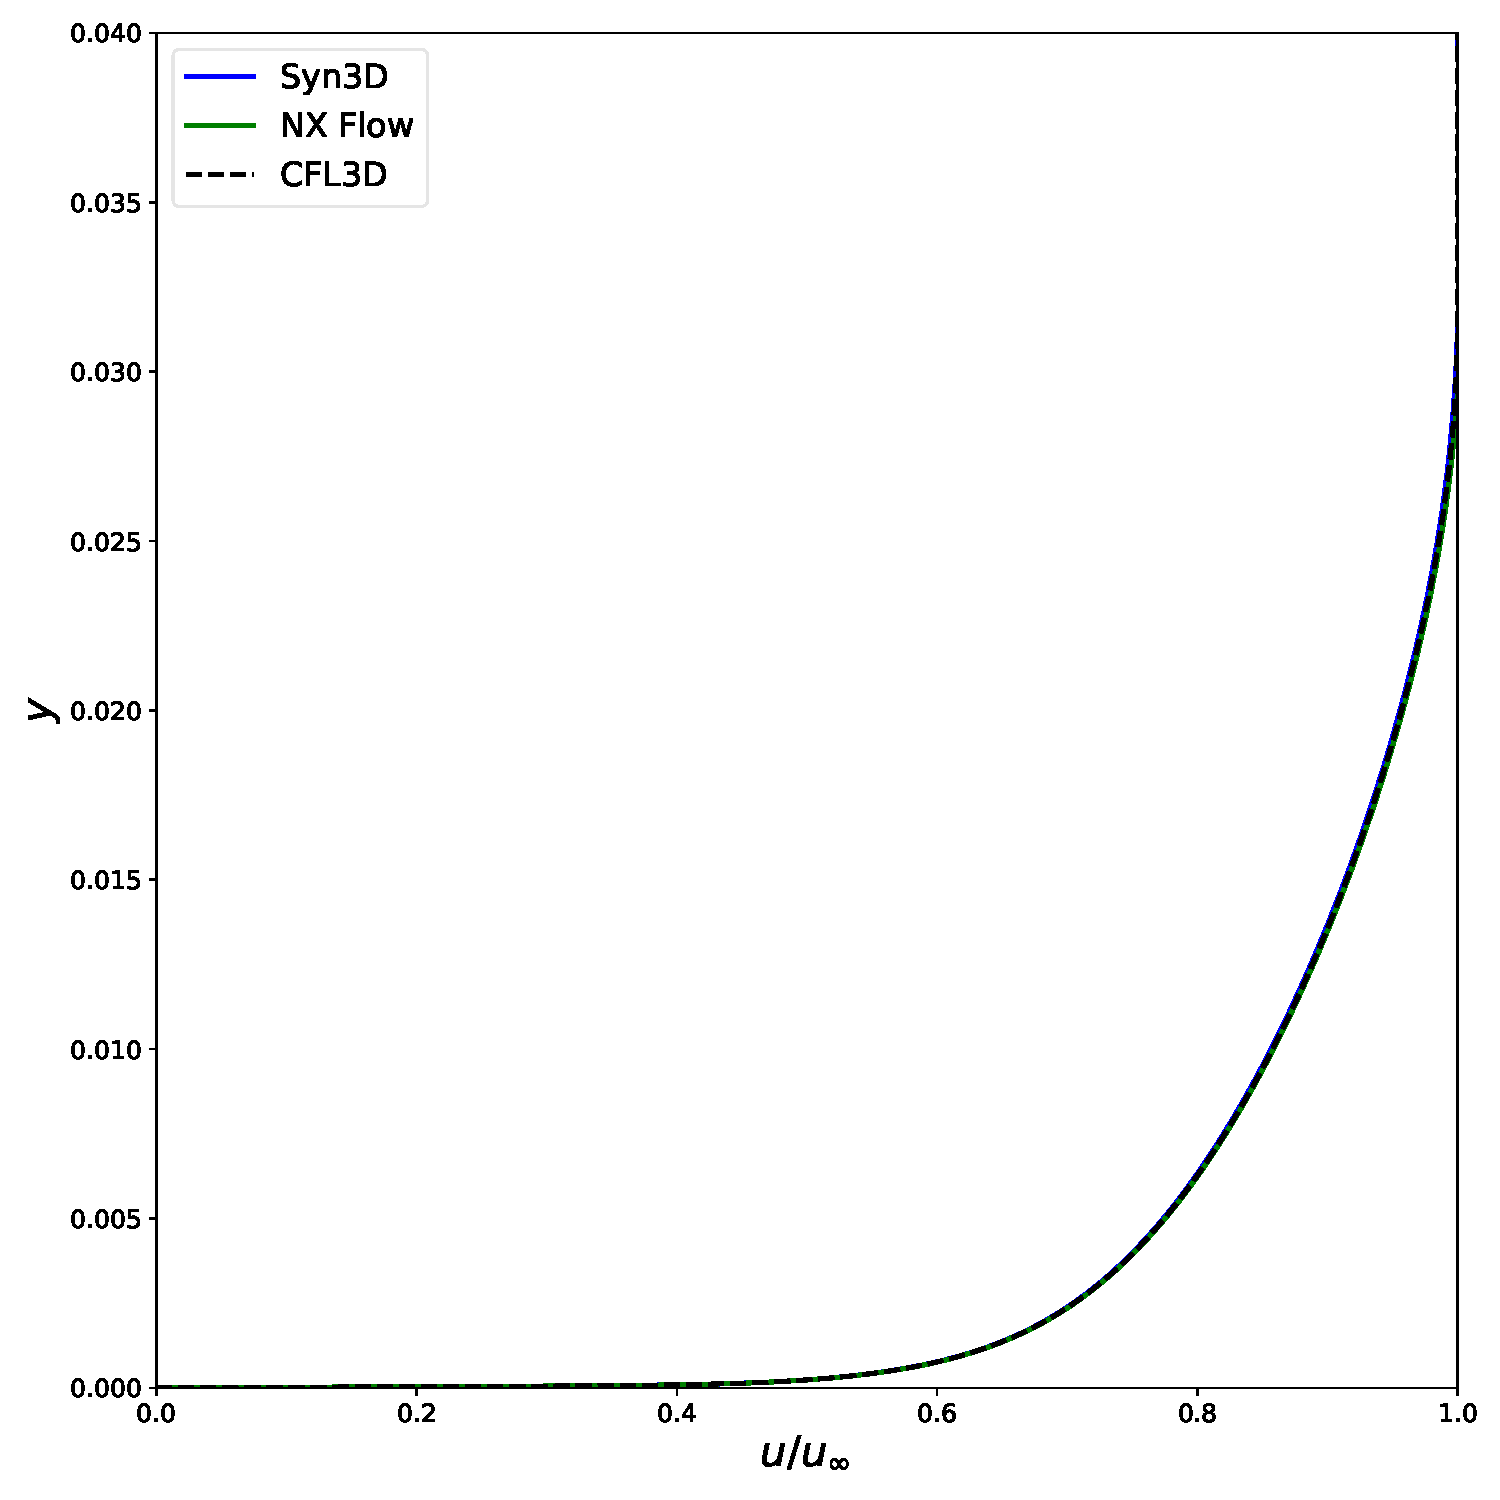
\includegraphics[width=1.0\textwidth]{figs/flat/u190.pdf}
  \caption{$x=1.90$}
\end{subfigure}
\caption{Flat Plate (syn3D \& NX Flow): $\frac{U}{U_{\infty}}$ profiles in the boundary layer}
\label{fig:flatu}
\end{figure}

\begin{figure}[ht!]
\centering
\begin{subfigure}{.45\textwidth}
  \centering
  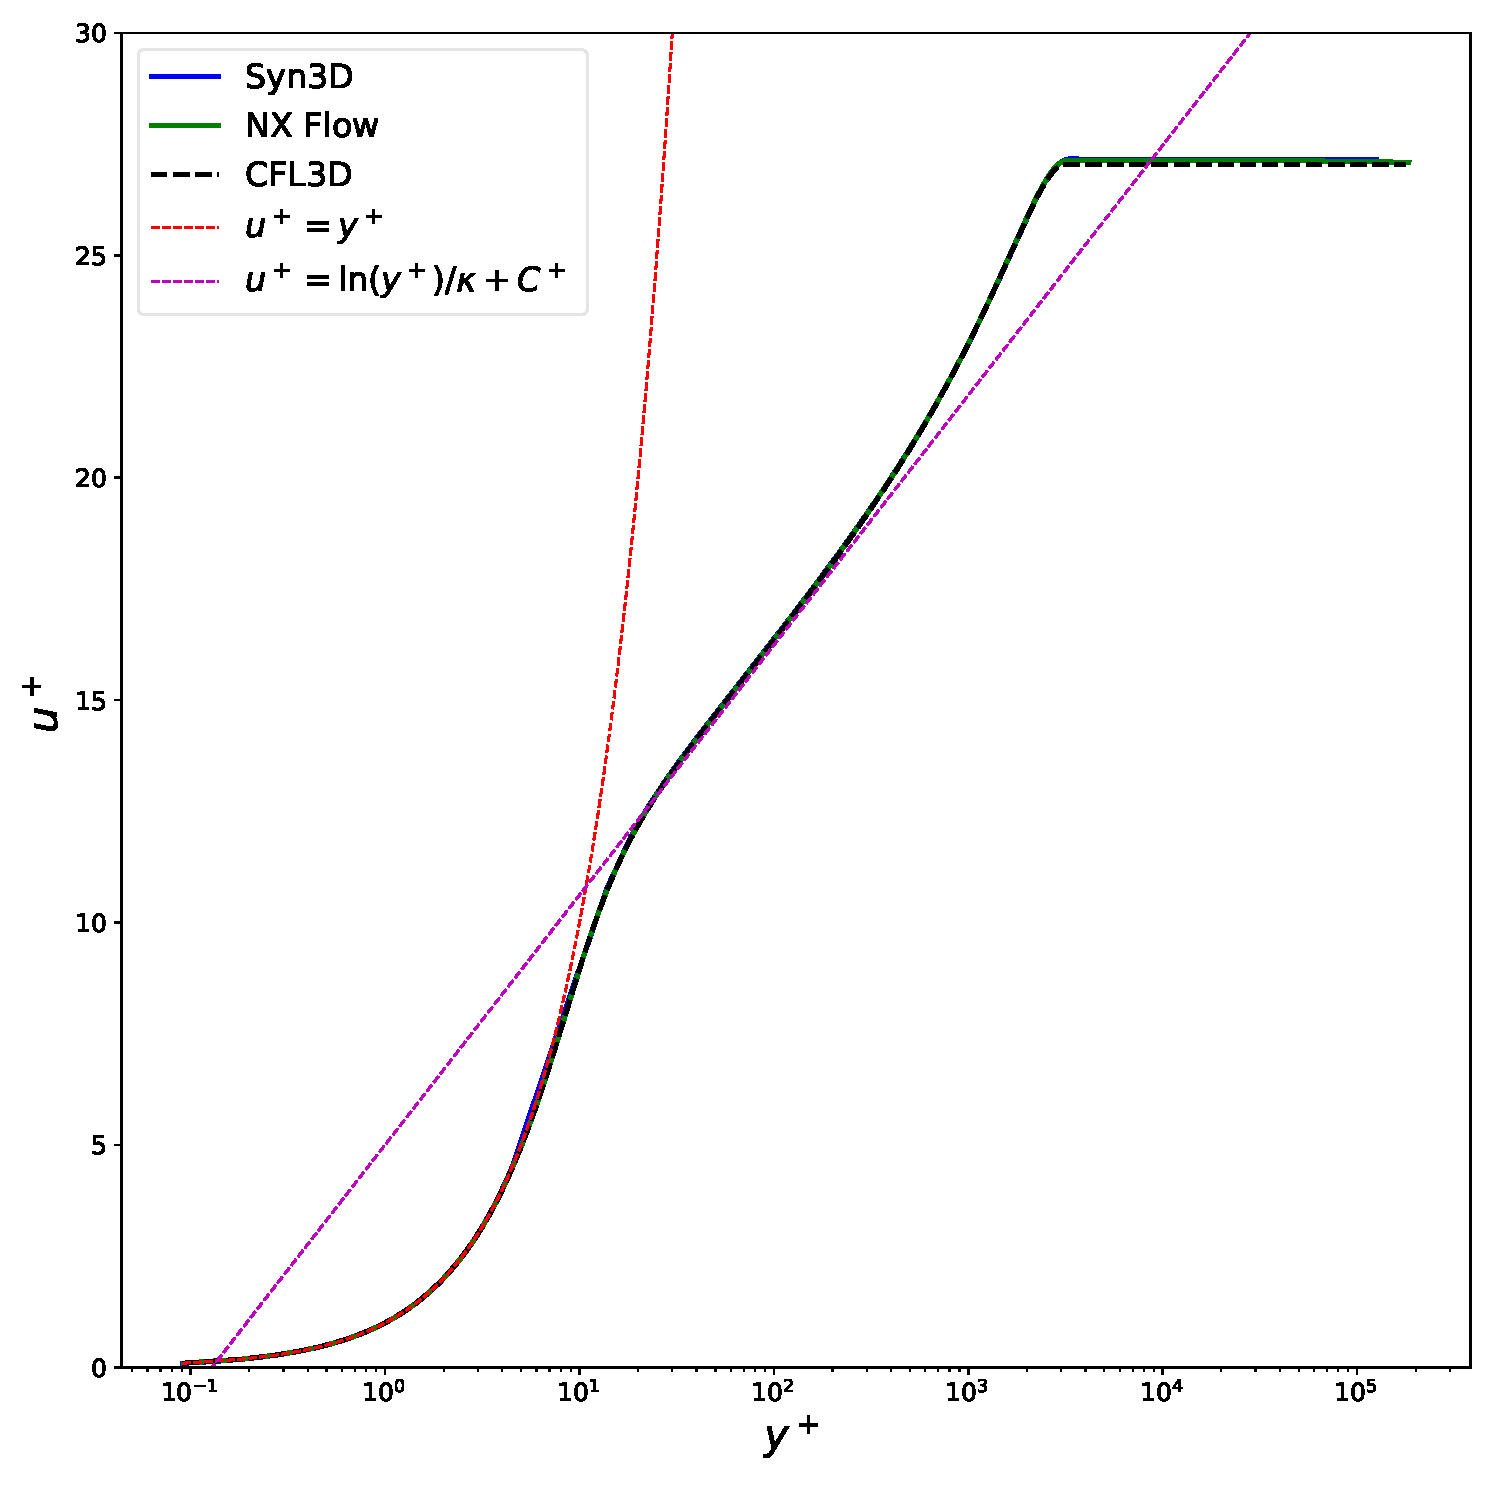
\includegraphics[width=1.0\textwidth]{figs/flat/uplus_yplus_097.pdf}
  \caption{$x=0.97$}
\end{subfigure}%
\begin{subfigure}{.45\textwidth}
  \centering
  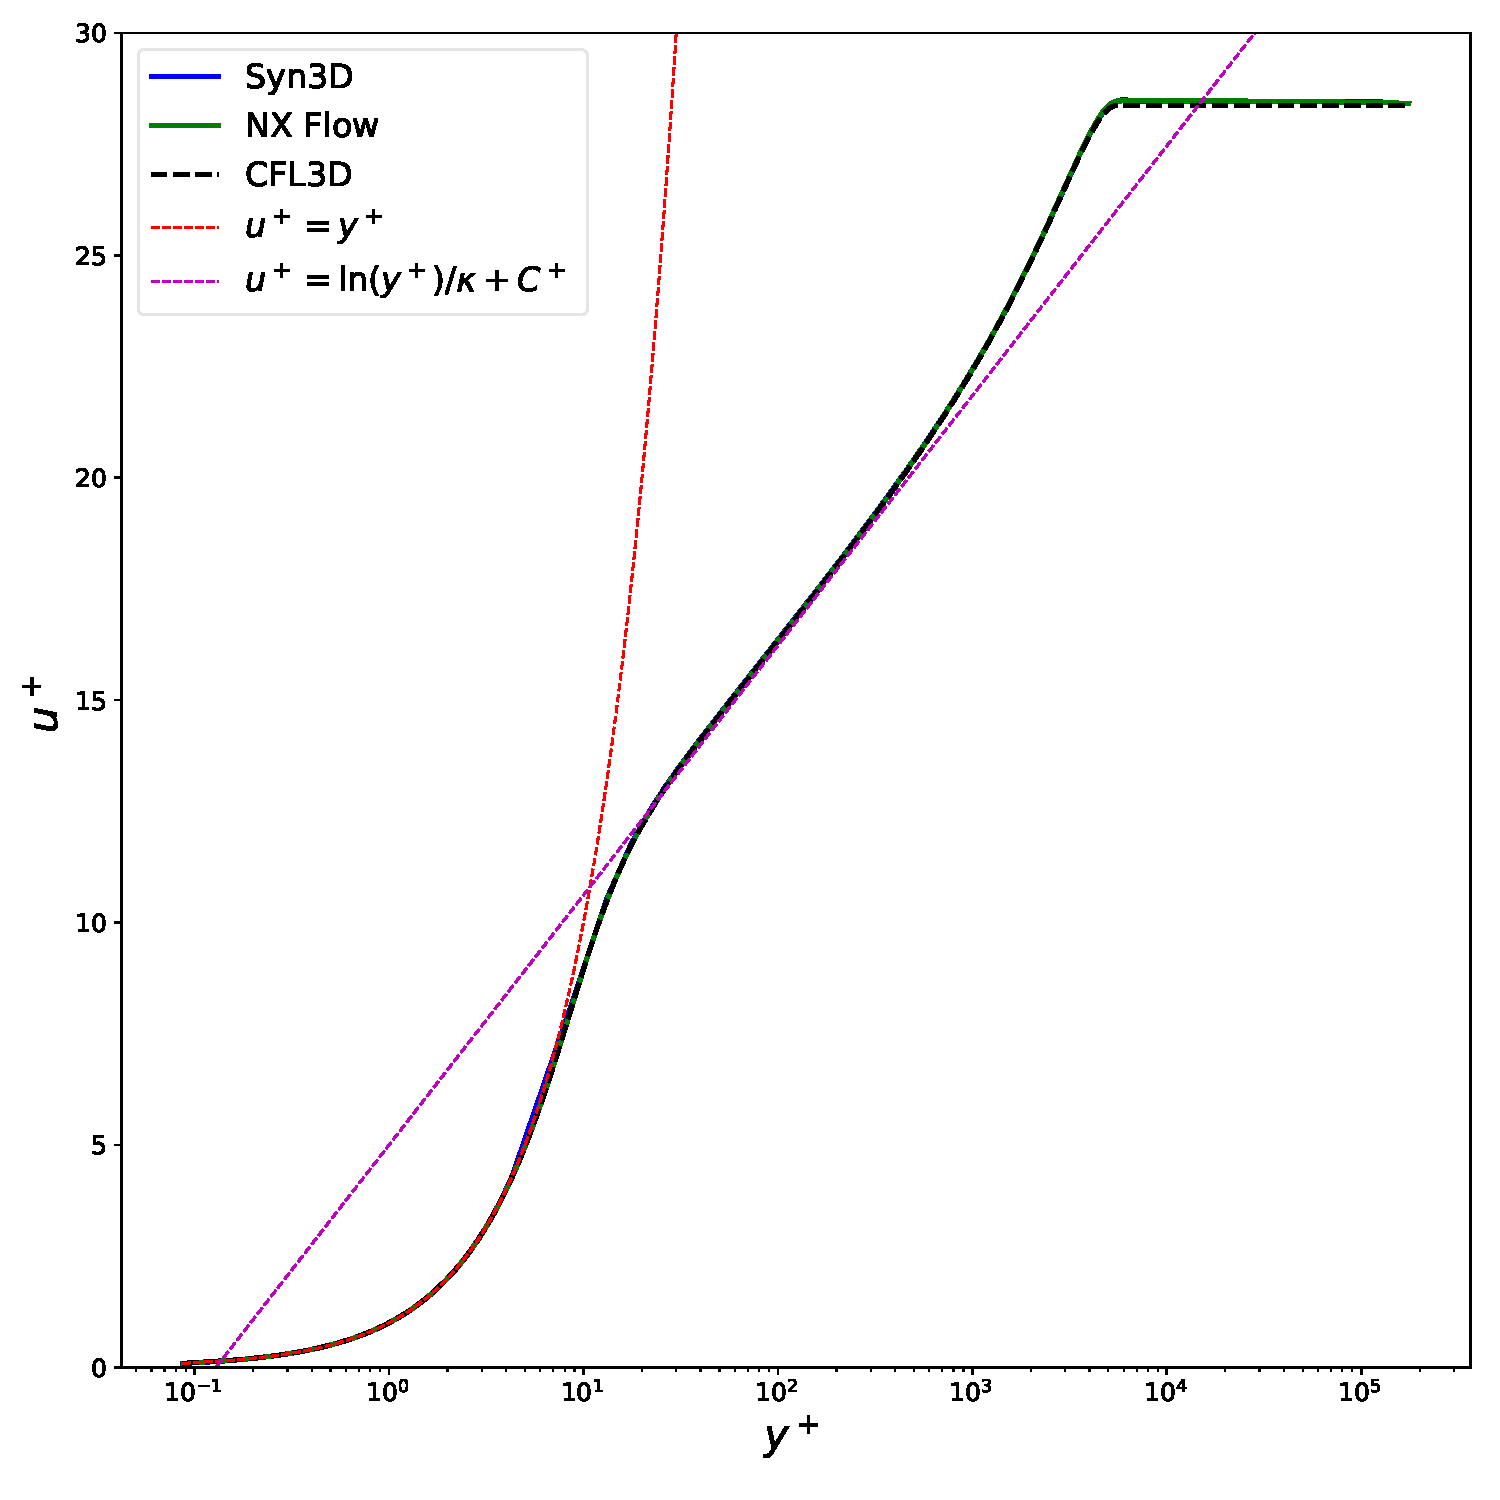
\includegraphics[width=1.0\textwidth]{figs/flat/uplus_yplus_190.pdf}
  \caption{$x=1.90$}
\end{subfigure}
\caption{Flat Plate (syn3D \& NX Flow): $u^+$ vs. $y^+$ profiles in the boundary layer. Law of the wall is also shown for comparison.}
\label{fig:flatupyp}
\end{figure}

\Cref{fig:flatforcestudy} shows the dependence of $C_D$ and $C_f$ on the grid spacing $h = 1/N^2$, where $N$ is the number of grid points. It can be seen that there is still significant differences in results between the second finest and finest grid for syn3D as compared to CFL3D and FUN3D -- the latter is a vertex-centered code also developed by NASA. Thus, syn3D may not have reached the asymptotic range of convergence. Moreover, the importance of a grid study can be seen from these plots: whereas results on the fine grid are mostly similar, they are quite different on the coarser grids, with some being over-predicted and others under-predicted compared to the asymptotic values.

The skin friction coefficient obtained by NX Flow is closer to that of FUN3D run in incompressible mode, which is higher than the compressible value. This explains the over-prediction in the skin friction coefficient as well as drag.

\Cref{fig:synflatcfstudy,fig:synflatprofilestudy} show the variation of skin friction coefficient along the plate and profiles of eddy viscosity and velocity with grid size respectively with syn3D and \Cref{fig:nxflatcfstudy,fig:nxflatprofilestudy} show the variation with NX Flow. These plots show that the solution field seems to converge to a unique solution, as opposed to oscillating back and forth between different values. As expected, solutions on coarser grids display increased dissipation; the discretization errors scale with the grid spacing and typically lead to increased diffusion. Moreover, the artificial dissipation parameters in syn3D were not tuned for each individual grid, and they lead to significantly increased dissipation on coarser grids. Nevertheless, the grid study provides an ability to determine the minimum required grid size to ensure sufficiently accurate values of the drag coefficient to within five drag counts. In the case of NX Flow, the $35\times25$ grid was required, while syn3D demanded a grid of $69\times49$. A study of the choice of artificial dissipation may reduce the grid density requirement, however, this was not part of the work.
\begin{figure}[ht!]
\centering
\begin{subfigure}{.45\textwidth}
  \centering
  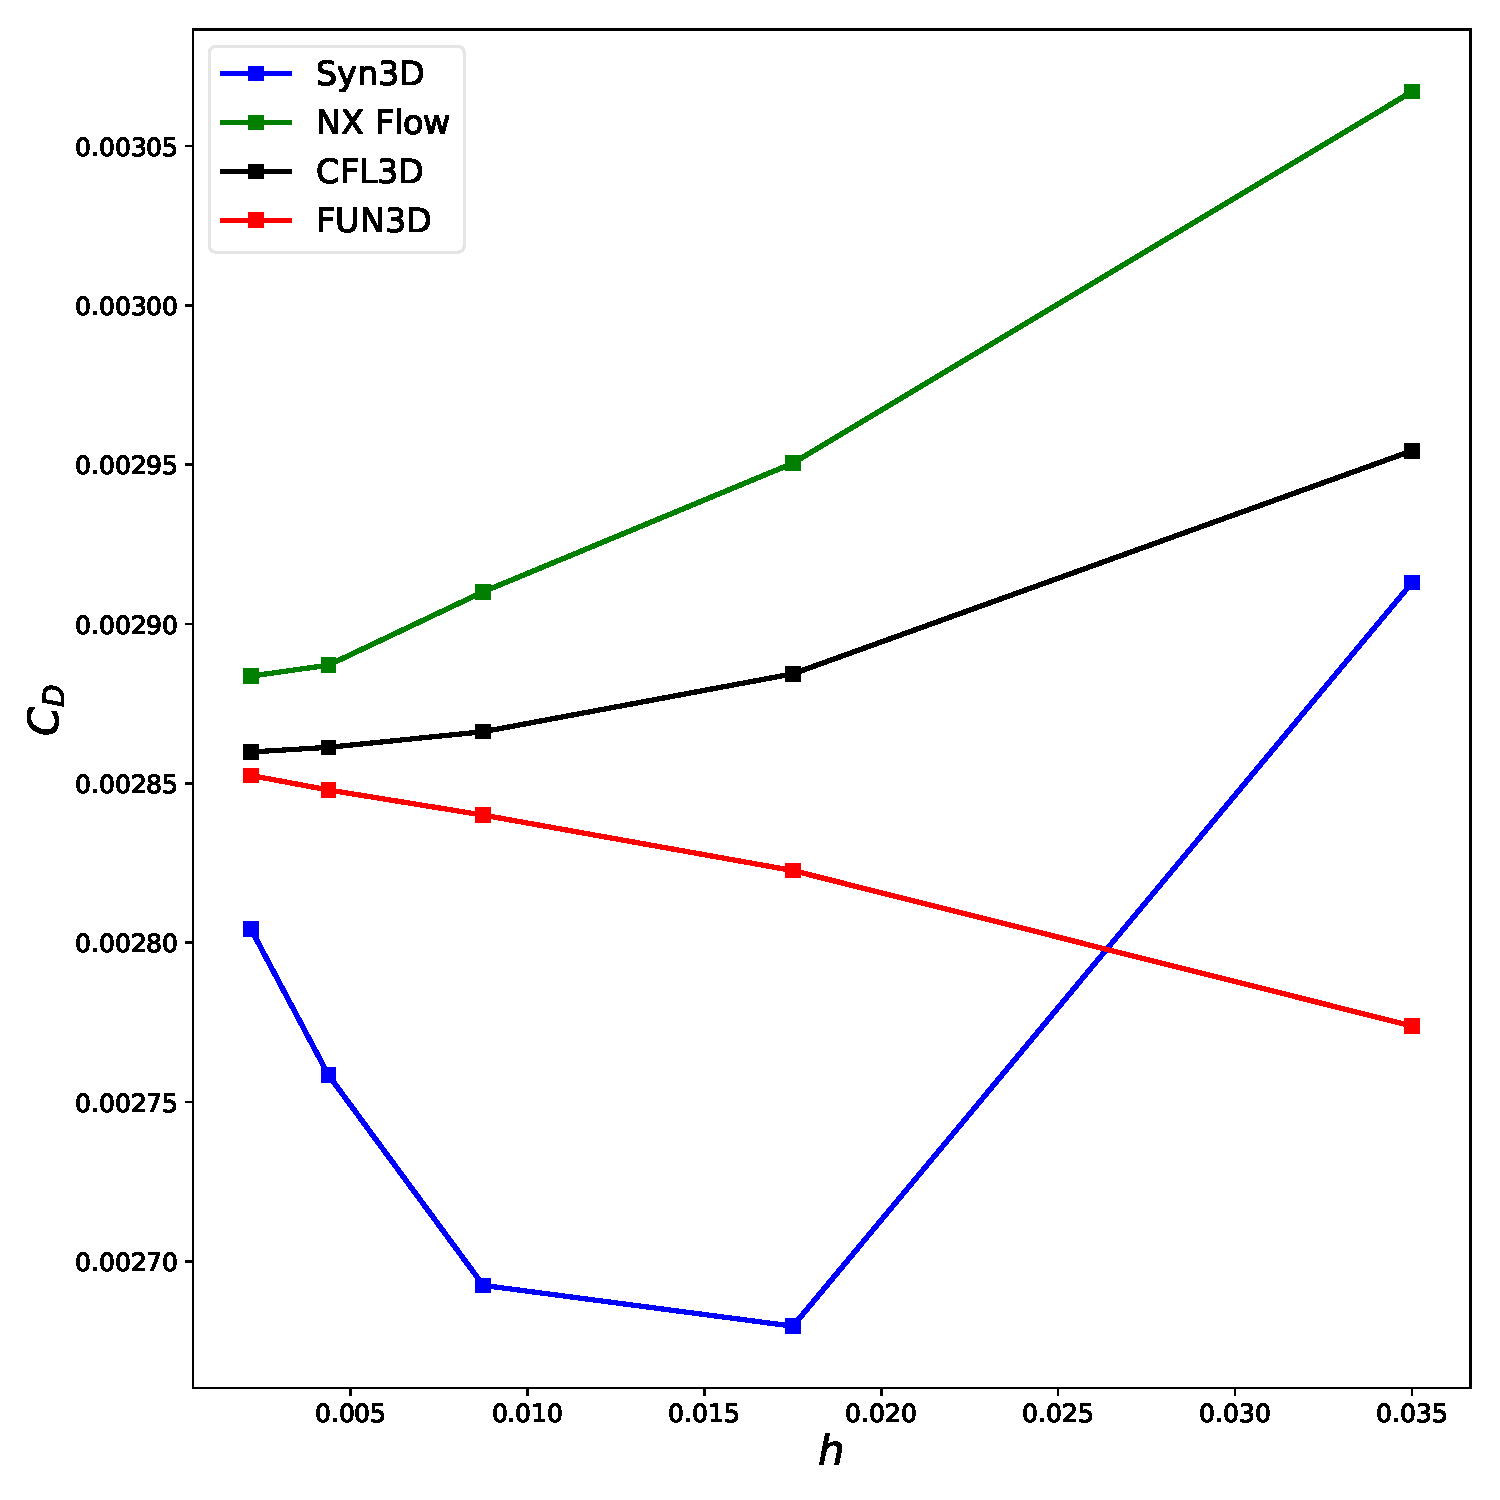
\includegraphics[width=1.0\textwidth]{figs/flat/cd_grid.pdf}
  \caption{Coefficient of drag.}
\end{subfigure}%
\begin{subfigure}{.45\textwidth}
  \centering
  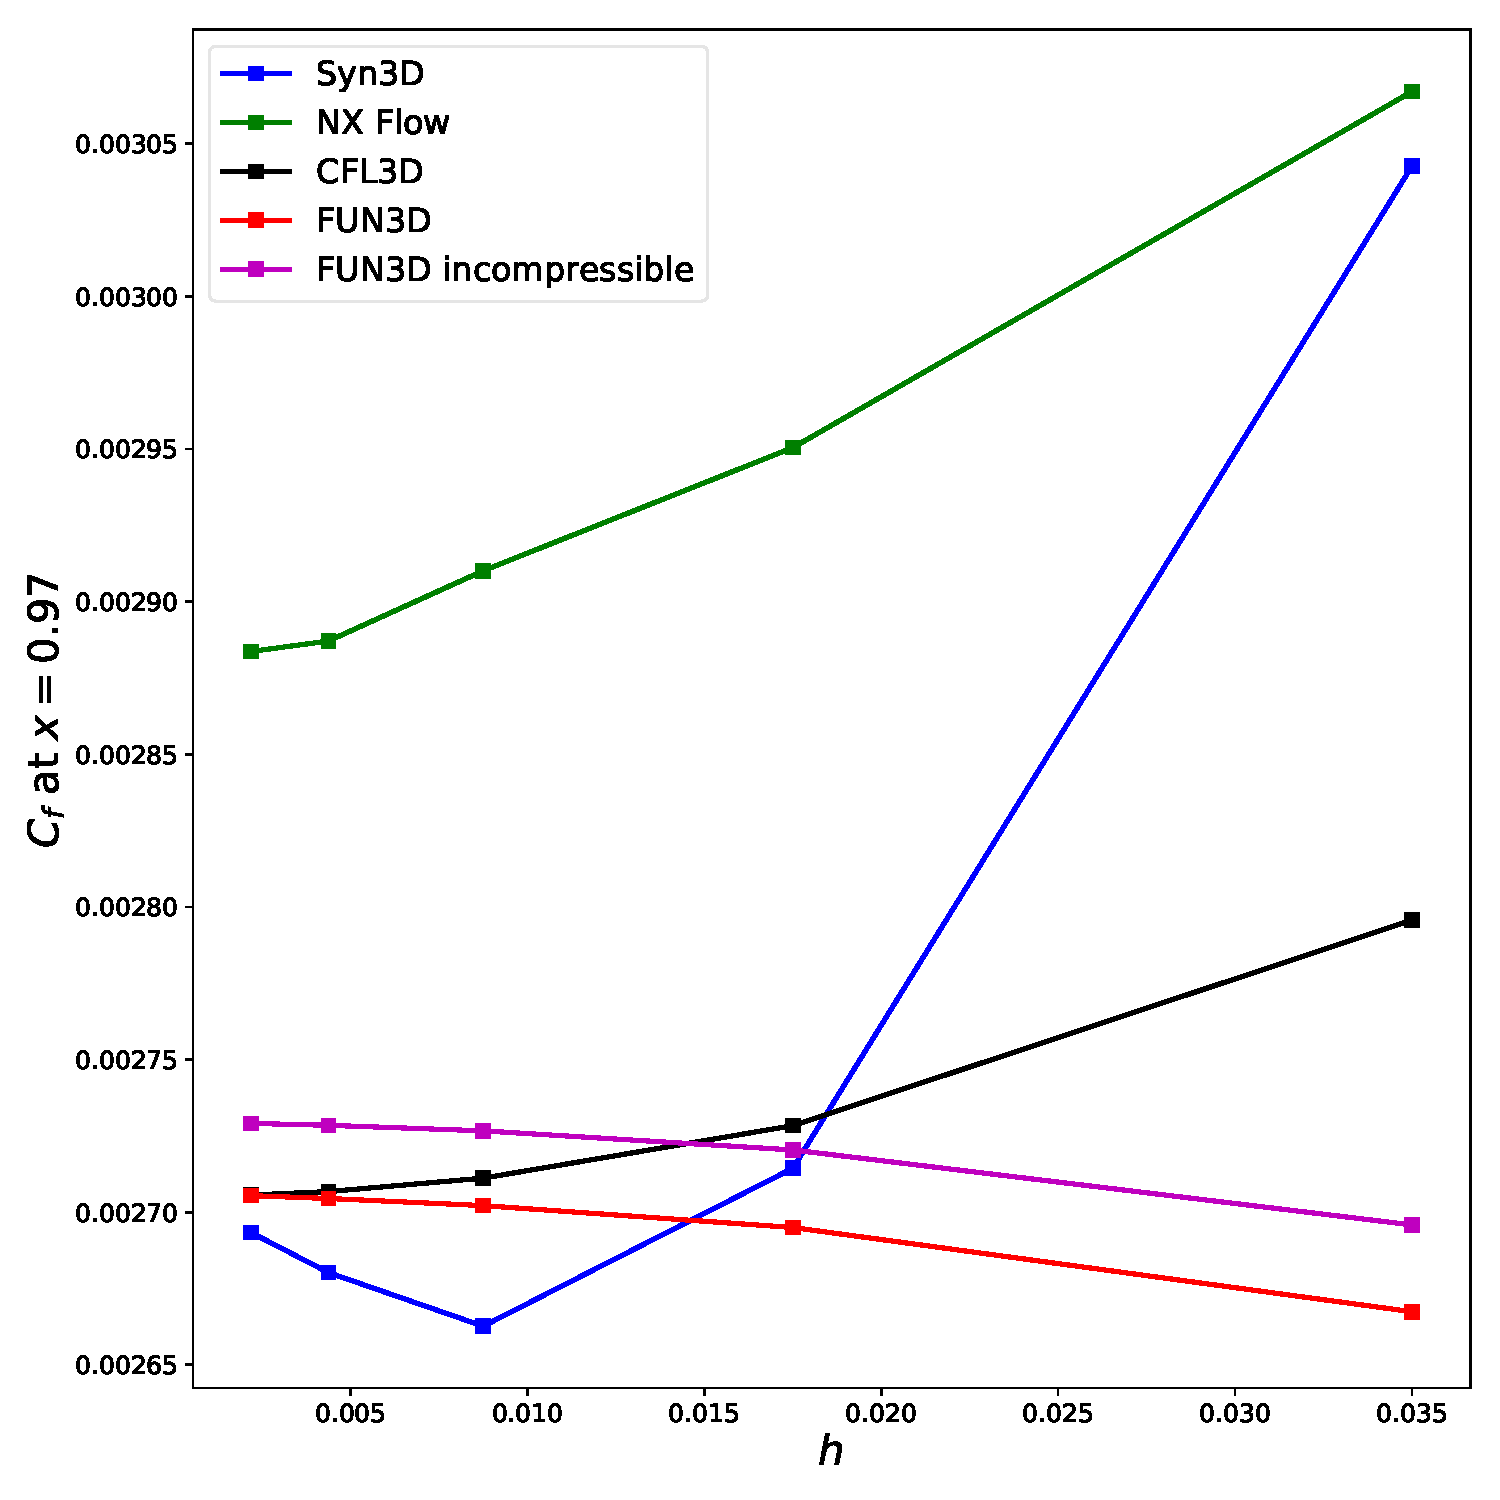
\includegraphics[width=1.0\textwidth]{figs/flat/cf_grid.pdf}
  \caption{Coefficient of Skin Friction at x=0.97.}
\end{subfigure}
\caption{Flat Plate (syn3D): Force coefficients for various grid sizes.}
\label{fig:flatforcestudy}
\end{figure}

\begin{figure}[ht!]
\centering
  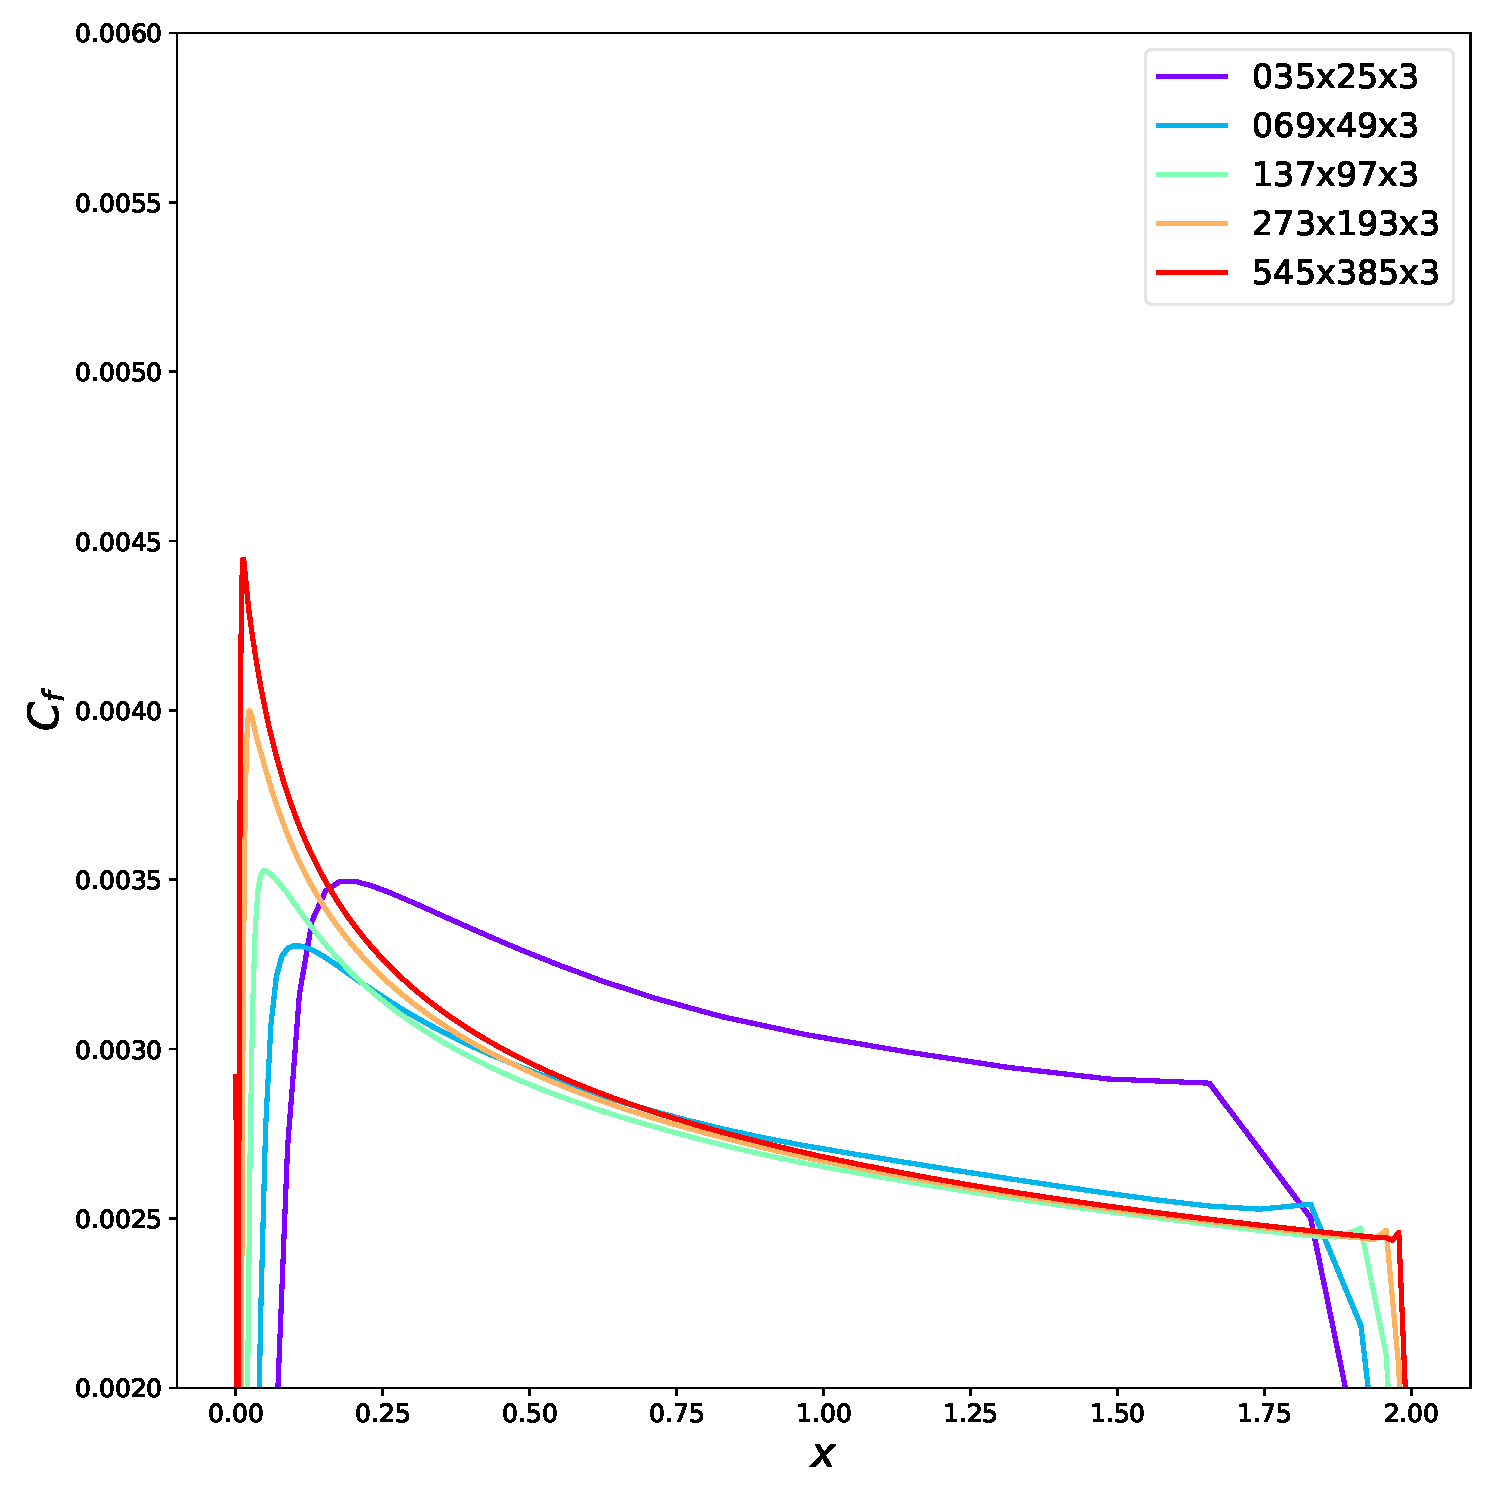
\includegraphics[width=0.7\textwidth]{figs/flat/skin_friction_grid.pdf}
  \caption{Flat Plate (syn3D): Coefficient of skin friction on various grids.}
  \label{fig:synflatcfstudy}
\end{figure}

\begin{figure}[ht!]
\centering
\begin{subfigure}{.45\textwidth}
  \centering
  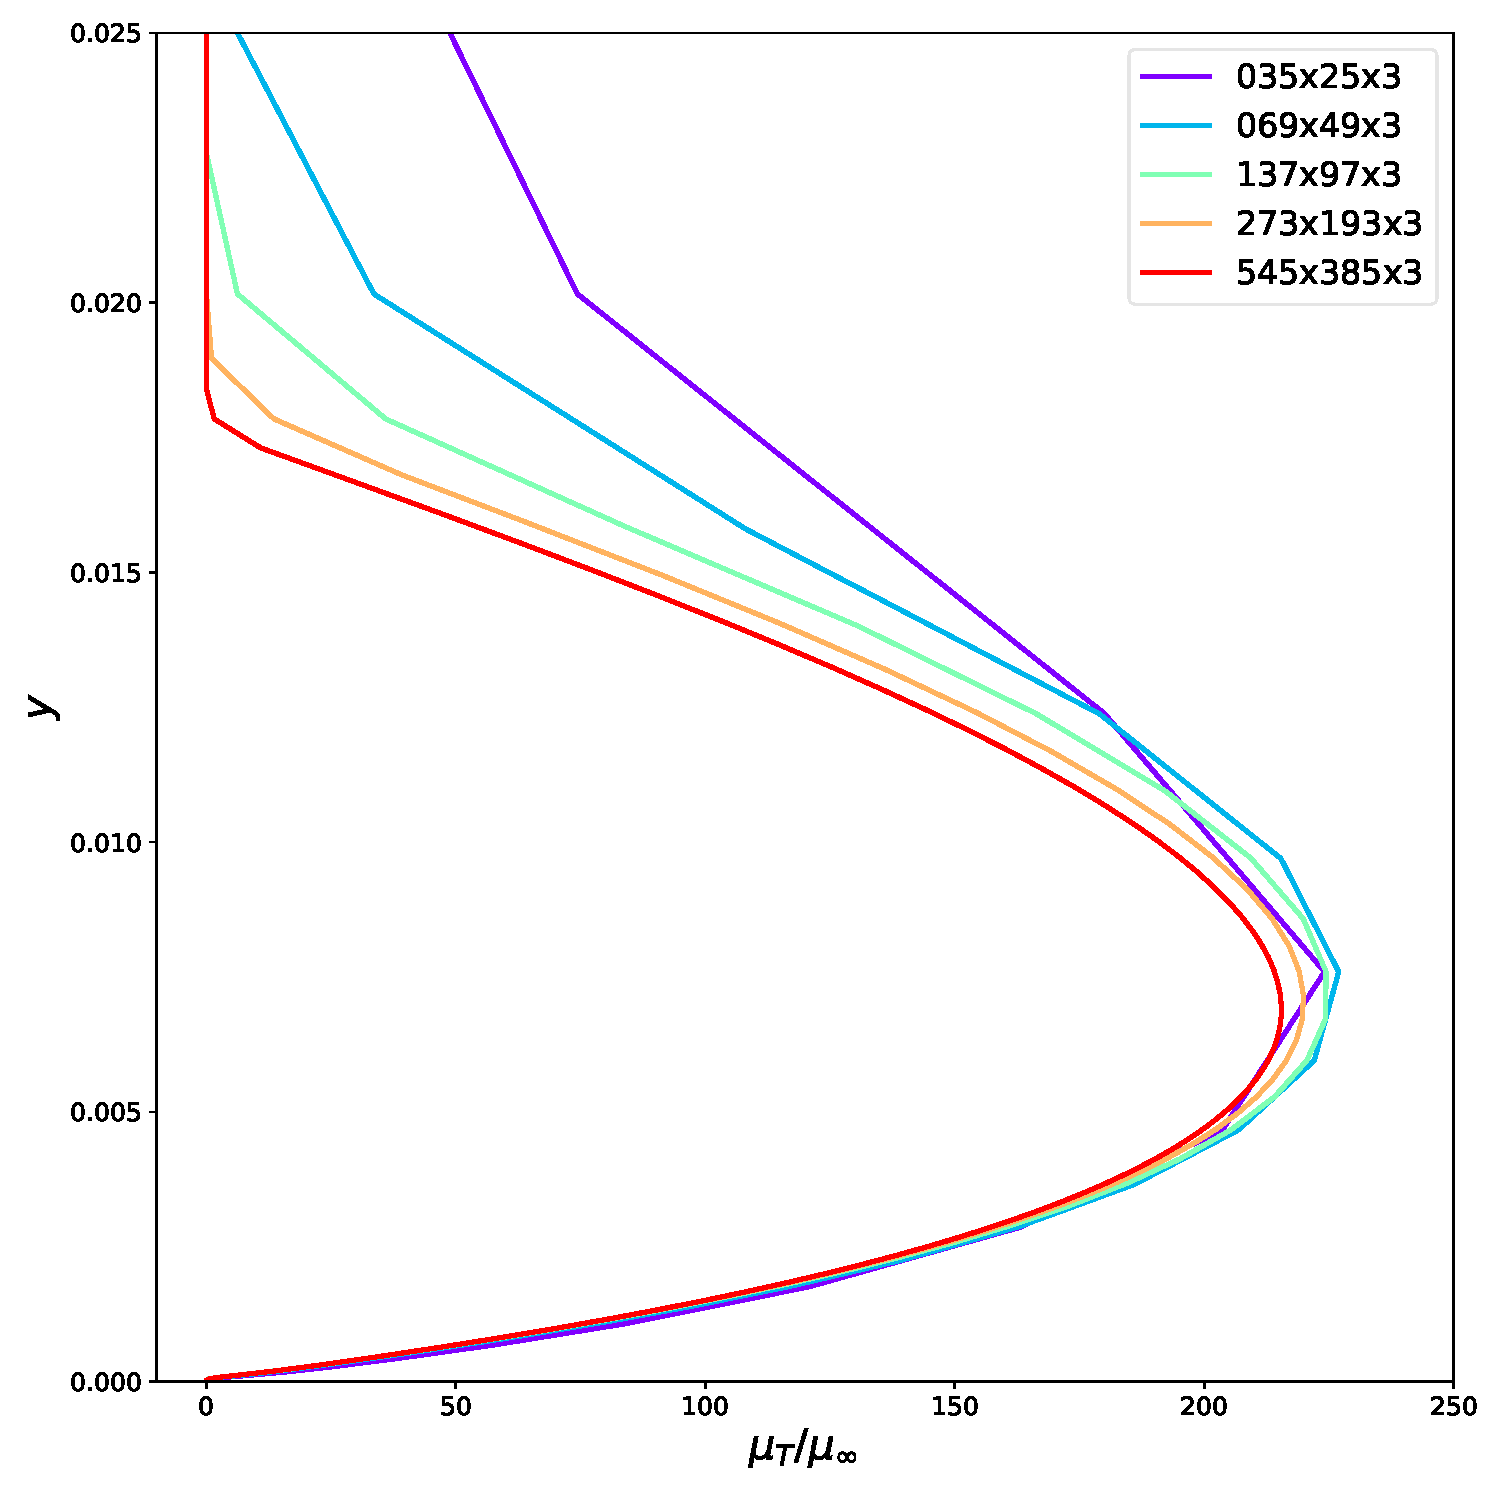
\includegraphics[width=1.0\textwidth]{figs/flat/rev_grid.pdf}
  \caption{Dimensionless eddy viscosity}
\end{subfigure}%
\begin{subfigure}{.45\textwidth}
  \centering
  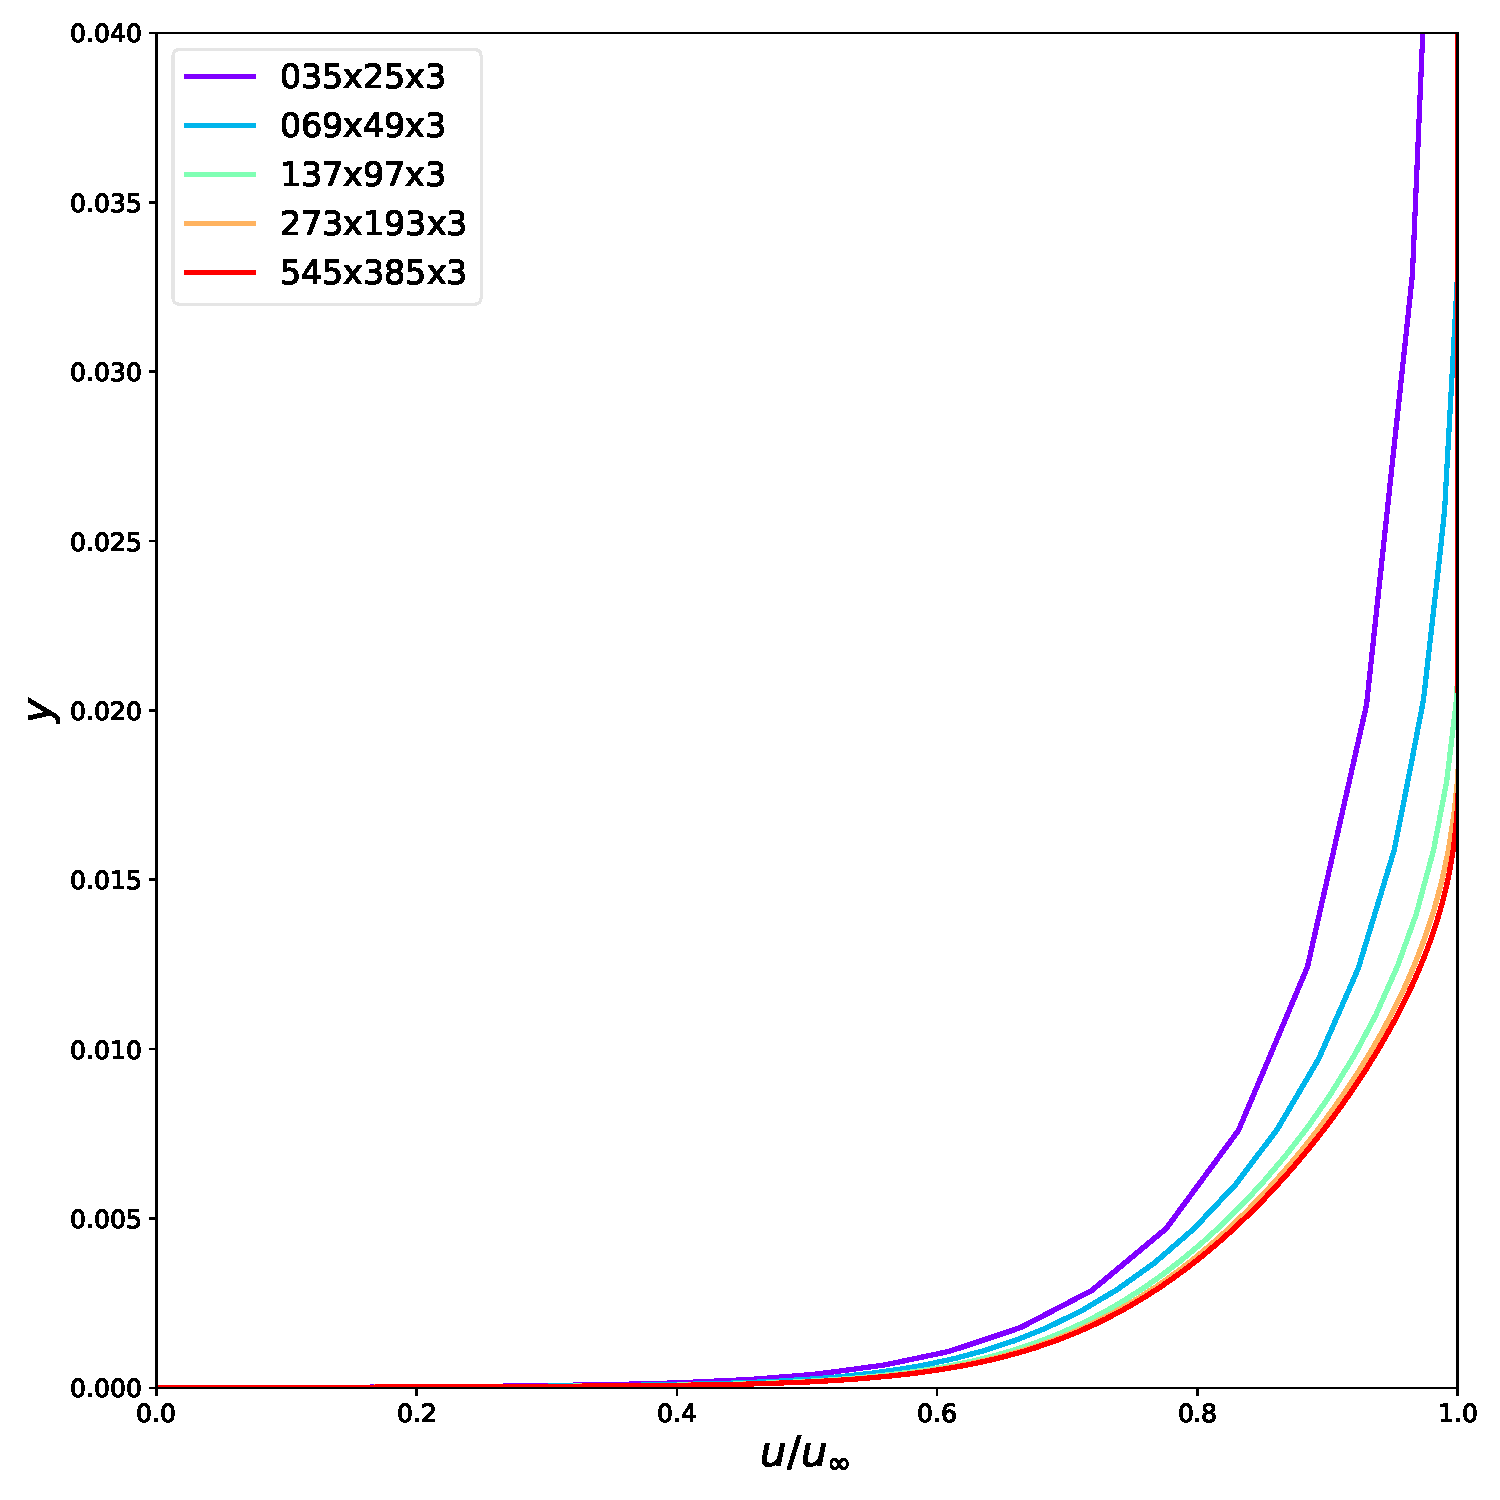
\includegraphics[width=1.0\textwidth]{figs/flat/u097_grid.pdf}
  \caption{Dimensionless velocity}
\end{subfigure}
\caption{Flat Plate (syn3D): Profiles at $x=0.97$ for various grid sizes.}
\label{fig:synflatprofilestudy}
\end{figure}

\begin{figure}[ht!]
\centering
  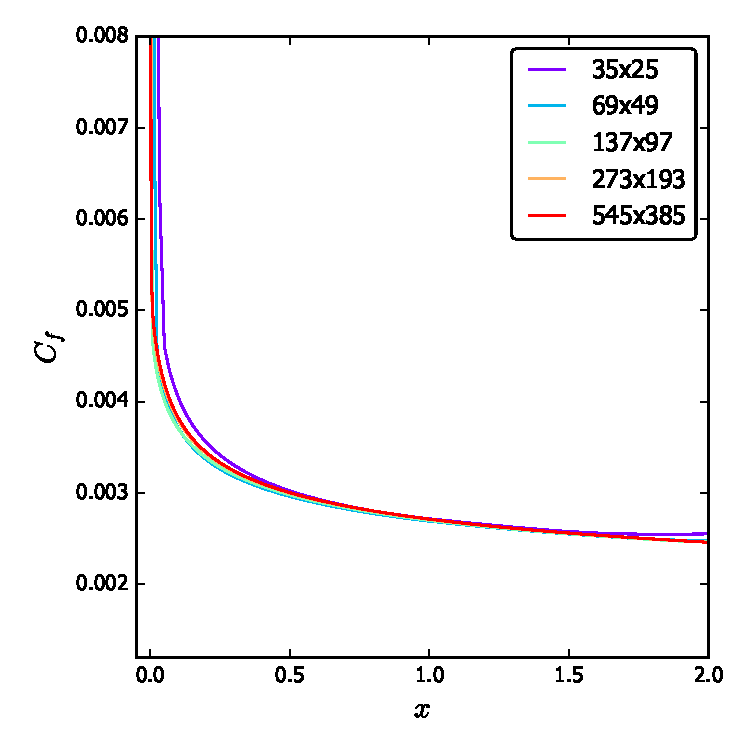
\includegraphics[width=0.7\textwidth]{figs/flatnx/cf_gridstudy.pdf}
  \caption{Flat Plate (NX Flow): Coefficient of skin friction on various grids.}
  \label{fig:nxflatcfstudy}
\end{figure}

\begin{figure}[ht!]
\centering
\begin{subfigure}{.45\textwidth}
  \centering
  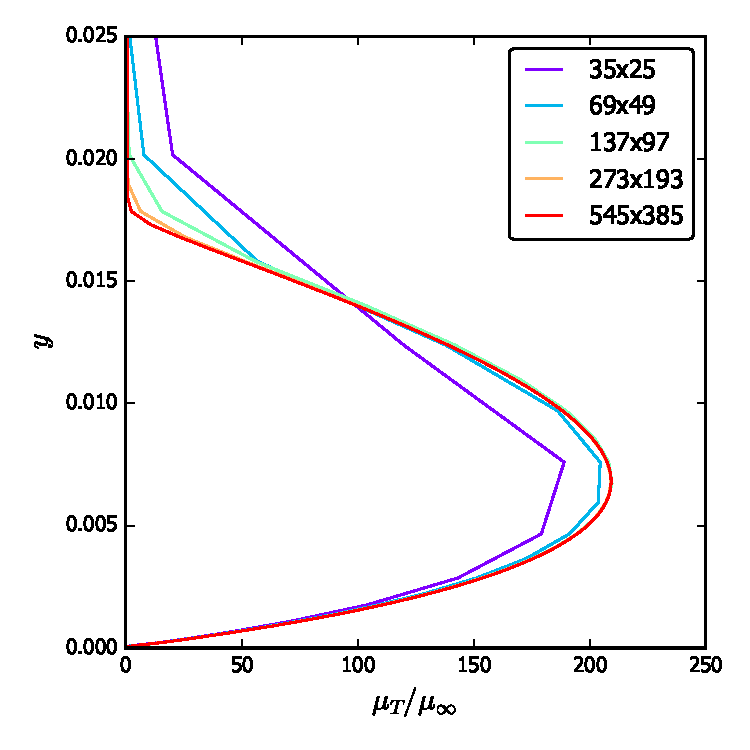
\includegraphics[width=1.0\textwidth]{figs/flatnx/mut_gridstudy.pdf}
  \caption{Dimensionless eddy viscosity}
\end{subfigure}%
\begin{subfigure}{.45\textwidth}
  \centering
  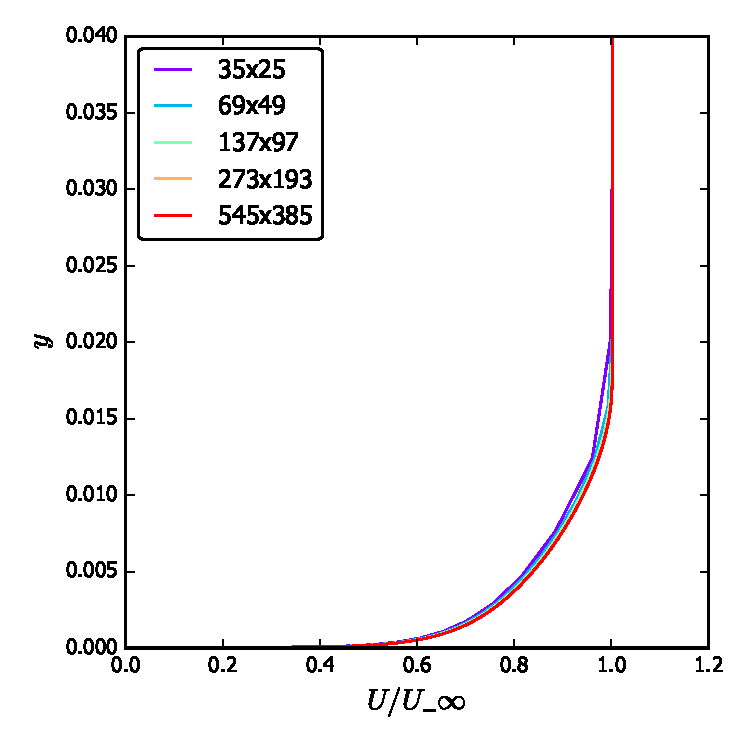
\includegraphics[width=1.0\textwidth]{figs/flatnx/u_x097_gridstudy.pdf}
  \caption{Dimensionless velocity}
\end{subfigure}
\caption{Flat Plate (NX Flow): Profiles at $x=0.97$ for various grid sizes.}
\label{fig:nxflatprofilestudy}
\end{figure}
